\documentclass[onecolumn, draftclsnofoot,10pt, compsoc]{IEEEtran}
\usepackage{amsmath}
\usepackage{amsthm}

\usepackage{alltt}
\usepackage{float}
\usepackage{color}

\usepackage{enumitem}

\usepackage{titling}
\usepackage{rotating}
\usepackage{pgfgantt}
\usepackage{graphicx}
\usepackage{xcolor}
\usepackage{anyfontsize}

\ganttset{group/.append style={orange},
milestone/.append style={red},
progress label node anchor/.append style={text=red}}
\usepackage{graphicx}
\usepackage{url}
\usepackage{setspace}
\usepackage{array}
\usepackage{tabu}
\usepackage{listings}
\usepackage{geometry}
\geometry{textheight=9.5in, textwidth=7in}
\graphicspath{ {images/} }
% 1. Fill in these details
\def \CapstoneTeamName{		Deep Learning on Embedded Platform}
\def \CapstoneTeamNumber{		14}
\def \GroupMemberOne{			Christopher Johnson}
\def \GroupMemberTwo{			Gabe Morey}
\def \GroupMemberThree{			Luay Alshawi}
\def \CapstoneProjectName{		AI Gaming}
\def \CapstoneSponsorCompany{	NVIDIA}
\def \CapstoneSponsorPerson{		Mark Ebersole}

\def \DocType{	%Problem Statement
				%Requirements Document
				%Technology Review
				%Design Document
				Progress Report
				}

\newcommand{\NameSigPair}[1]{\par
\makebox[2.75in][r]{#1} \hfil 	\makebox[3.25in]{\makebox[2.25in]{\hrulefill} \hfill		\makebox[.75in]{\hrulefill}}
\par\vspace{-12pt} \textit{\tiny\noindent
\makebox[2.75in]{} \hfil		\makebox[3.25in]{\makebox[2.25in][r]{Signature} \hfill	\makebox[.75in][r]{Date}}}}

\begin{document}
\begin{titlepage}
    \pagenumbering{gobble}
    \begin{singlespace}
    	% 
\includegraphics[height=4cm]{coe_v_spot1}
        \hfill
        % 4. If you have a logo, use this includegraphics command to put it on the coversheet.
        %\includegraphics[height=4cm]{CompanyLogo}
        \par\vspace{.2in}
        \centering
        \scshape{
            \huge CS Capstone \DocType \par
            {\large\today}\par
            \vspace{.5in}
            \textbf{\Huge\CapstoneProjectName}\par
			\vfill
            {\large Prepared for}\par
            \Huge \CapstoneSponsorCompany\par
            \vspace{5pt}
            {\Large\NameSigPair{\CapstoneSponsorPerson}\par}
            {\large Prepared by }\par
            Group\CapstoneTeamNumber\par
            % 5. comment out the line below this one if you do not wish to name your team
            \CapstoneTeamName\par
            \vspace{5pt}
			{\Large
                \NameSigPair{\GroupMemberOne}\par
                \NameSigPair{\GroupMemberTwo}\par
                \NameSigPair{\GroupMemberThree}\par
            }
            \vspace{20pt}
        }
        \begin{abstract}
        In this document we describe everything we have done in our project to create a deep learning program that can learn to play the game Galaga.
	The project was created to be used as a training tool for NVIDIA's Deep Learning Institute.
	This document covers every piece of development material, including previously created documents, changes, and the final design of the project.
	Each team member will also present their logs of the development process and a summary of their learning throughout the term.



        \end{abstract}
    \end{singlespace}
\end{titlepage}

\newpage
\pagenumbering{arabic}
\tableofcontents

\section{Introduction}
Our project was requested by NVIDIA's Deep Learning Institute in order to provide a new training course in neural network training and development for new developers.
The goal was to provide an exciting project for beginners that would help ease them in to the growing field of Deep Learning.
Deep Learning itself is a field focused on the training and development of Deep Neural networks to be applied to machine-learning based challenges.
Deep Learning is a major avenue toward building technology like self-driving cars and autmoatic facial recognition. 
Getting more developers involved will support the field's continued growth and lead to important breakthroughs in AI technology.
\newline\newline
The project itself was given in an open-ended fashion.
We, as a team, were allowed to choose a project that met a few simple requirements.
The first was that we had to use a Neural Network to accomplish the task. 
The second was that it had to run inference on the Jetson TX1 developer kit.
With these guidelines set, we decided to use the project to train a neural network to play the video game Galaga, an arcade shooter.
\newline\newline
Our client was Mark Ebersole and our team consisted of Gabriel Morey, Luay Alshawi, and Chris Johnson. 
Mr. Ebersole acted as a supervisor and provided us necessary resources from his company, such as the Jetson TX1 developer kit.
He also connected us with people at NVIDIA who could offer advice on technical implementation of the project.
Chris was assigned as team captain and provided work building training images, setting up and acquiring hardware, and creating and organizing documentation.
Luay was the primary authority on the neural network itself and was in charge of training it and improving its functionality for our task.
Gabriel worked on training images, device communication, neural network functionality improvements, deployment testing, and documentation improvements.

%\section{Requirements document}

%%Copyright 2014 Jean-Philippe Eisenbarth
%This program is free software: you can
%redistribute it and/or modify it under the terms of the GNU General Public
%License as published by the Free Software Foundation, either version 3 of the
%License, or (at your option) any later version.
%This program is distributed in the hope that it will be useful,but WITHOUT ANY
%WARRANTY; without even the implied warranty of MERCHANTABILITY or FITNESS FOR A
%PARTICULAR PURPOSE. See the GNU General Public License for more details.
%You should have received a copy of the GNU General Public License along with
%this program.  If not, see <http://www.gnu.org/licenses/>.

%Based on the code of Yiannis Lazarides
%http://tex.stackexchange.com/questions/42602/software-requirements-specification-with-latex
%http://tex.stackexchange.com/users/963/yiannis-lazarides
%Also based on the template of Karl E. Wiegers
%http://www.se.rit.edu/~emad/teaching/slides/srs_template_sep14.pdf
%http://karlwiegers.com
% \documentclass[letterpaper,10pt]{article}
\documentclass{scrreprt}
\usepackage{listings}
\usepackage{underscore}
\usepackage[bookmarks=true]{hyperref}
\usepackage[utf8]{inputenc}
\usepackage[english]{babel}
\usepackage{graphicx}
\usepackage{amssymb}
\usepackage{amsmath}
\usepackage{amsthm}

\usepackage{alltt}
\usepackage{float}
\usepackage{color}
\usepackage{url}

\usepackage{enumitem}

\usepackage{geometry}

\usepackage{titling}
\usepackage{rotating}
\usepackage{pgfgantt}
\usepackage{graphicx}
\usepackage{xcolor}
\usepackage{anyfontsize}

\ganttset{group/.append style={orange},
milestone/.append style={red},
progress label node anchor/.append style={text=red}}

\geometry{textheight=8.5in, textwidth=6in}
\hypersetup{
    bookmarks=false,    % show bookmarks bar?
    pdftitle={Software Requirement Specification},    % title
    pdfauthor={Jean-Philippe Eisenbarth},                     % author
    pdfsubject={TeX and LaTeX},                        % subject of the document
    pdfkeywords={TeX, LaTeX, graphics, images}, % list of keywords
    colorlinks=true,       % false: boxed links; true: colored links
    linkcolor=blue,       % color of internal links
    citecolor=black,       % color of links to bibliography
    filecolor=black,        % color of file links
    urlcolor=purple,        % color of external links
    linktoc=page            % only page is linked
}%
\def\myversion{1.0 }
\date{}
%\title
\usepackage{hyperref}
\begin{document}

\begin{flushright}
    \rule{16cm}{5pt}\vskip1cm
    \begin{bfseries}
        \Huge{SOFTWARE REQUIREMENTS\\ SPECIFICATION}\\
        \vspace{1.9cm}
        for\\
        \vspace{1.9cm}
        Deep Learning on Embedded Platform\\
        \vspace{1.9cm}
        \LARGE{Version \myversion}\\
        \vspace{1.9cm}
        Prepared by Christopher Johnson, Luay Alshawi, Gabe Morey\\
        \vspace{1.9cm}
        CS 461\\
        \vspace{1.9cm}
        \today\\
    \end{bfseries}
\end{flushright}

\tableofcontents


\chapter{Introduction}

\section{Purpose}

The goal of this document is to create a clear requirements documentation that identifies the necessary parts to \
accomplish this project.
The main requirements are to run a deep learning application on the Jetson TX1 development kit and to have docume\
ntation clear enough to recreate our project.
The end result of this project will be an AI capable of playing the game Galaga, and the project itself will be u\
sed by Nvidia to create a lesson for their deep learning institute.
Since the lesson plan will not be developed by us, this document only covers the project requirements and not requi\
rements for the lesson.

\section{Scope}

The project name will be AI Gaming and the solution of our project will need to be able to beat the first level of the game at least 90\% of the time.
Ideally the system should be able to make it past level five approximately 50\% of the time.
The ability of the system to make it farther than that on average, or to increase the percent chance on it making it to certain points, will be considered a stretch goal.

\section{Definitions, acronyms, and abbreviations}
JETSON TX1 Developer Kit: Tiny computer which has a full-featured development platform for visual computing.
\newline
AI: A branch of computer science dealing with the simulation of intelligent behavior in computers.

\section{References}
N. C. L. Information, Deep learning, NVIDIA Developer, 2016. [Online]. Available: https://developer.nvidia.com/deep-learning. Accessed: Oct. 18, 2016.\newline
NVIDIA, 2016. [Online]. Available: http://www.nvidia.com/object/jetson-tx1-dev-kit.html. Accessed: Nov. 2, 2016.\newline
Merriam-Webste, 2016. [Online]. Available: http://www.merriam-webster.com/dictionary/artificial%20intelligence. Accessed: Nov. 2, 2016.

\chapter{Overall Description}

\section{Product perspective}
Open...
\section{Product Functions}

The project goal is to teach a neural net to play a video game.
The neural net will take video input and use it to learn how to play the game Galaga.
A camera or screen capture device must be used to retrieve game state input.
The neural net must be trained and allowed to create its own code to accomplish the task.
The neural network should define for itself how to respond to in-game stimuli and react accordingly, as per the training it has received.
We may code interactions between the net and the game to allow it to play the game.
We may not hard code its responses to in-game stimuli, as these responses must be trained into the neural net.
The final project must be able to run inference on the Jetson TX1 developer platform.

\section{User characteristics}
Open...
\section{Constraints}
Open...
\section{Assumptions and dependencies}
Open...

\chapter{Chart}
\section{Timeline}
\resizebox{\textwidth}{!}{

%    \centering
     \begin{ganttchart}[%Specs
     y unit title=2cm,
     y unit chart=2cm,
     vgrid,hgrid,
     title height=1,
%     title/.style={fill=none},
     title label font=\bfseries\footnotesize,
     bar/.style={fill=blue},
     bar height=0.7,
%   progress label text={},
     group right shift=0,
     group top shift=0.7,
     group height=.3,
     group peaks width={0.2},
     inline]{1}{50}
    %labels
    \gantttitle{Plan}{50}\\  % title 1
    \gantttitle{W1}{2}
    \gantttitle{W2}{2}
    \gantttitle{W3}{2}
    \gantttitle{W4}{2}
    \gantttitle{W5}{2}
    \gantttitle{W6}{2}
    \gantttitle{W7}{2}
    \gantttitle{W8}{2}
    \gantttitle{W9}{2}
    \gantttitle{W10}{2}
    \gantttitle{W11}{2}
    \gantttitle{W12}{2}
    \gantttitle{W13}{2}
    \gantttitle{W14}{2}
    \gantttitle{W15}{2}
    \gantttitle{W16}{2}
    \gantttitle{W17}{2}
    \gantttitle{W18}{2}
    \gantttitle{W19}{2}
    \gantttitle{W20}{2}
    \gantttitle{W21}{2}
    \gantttitle{W22}{2}
    \gantttitle{W23}{2}
    \gantttitle{W24}{2}
    \gantttitle{W25}{2}
    % Setting group if any
    \ganttgroup[inline=false]{Documents}{1}{16} \\
    \ganttbar[progress=30,inline=false]{Requirement}{1}{5} \\
    \ganttbar[progress=0,inline=false]{Technical}{5}{10}\\
    \ganttbar[progress=0,inline=false]{Design}{10}{15} \\

    \ganttgroup[inline=false]{\small  {Winter Break} } {17}{24} \\

    \ganttgroup[inline=false]{\small{Desing Game Interface}}{25}{30} \\

    \ganttgroup[inline=false]{\small{Train Neural Network}}{31}{39} \\
    \ganttbar[progress=0,inline=false]{Training 1}{31}{33}\\
    \ganttbar[progress=0,inline=false]{Training 2}{34}{36}\\
    \ganttbar[progress=0,inline=false]{Training 3}{37}{39}\\

    \ganttgroup[inline=false]{Game Testing}{31}{39} \\
    \ganttbar[progress=0,inline=false]{Test 1}{32}{33}\\
    \ganttbar[progress=0,inline=false]{Test 2}{35}{36}\\
    \ganttbar[progress=0,inline=false]{Test 3}{38}{41}\\

    \ganttgroup[inline=false]{Improvements}{42}{50} \\

\end{ganttchart}
%    \caption{Gantt diagram for 2013--2014 Project}
%\end{figure}
}

\end{document}


\section{Changes made from the requirements document}
\subsection{Change Table}
\begin{center}
\begin{tabu} to 0.9\linewidth{ || X[l] | X[l] | X[l] | X[l] || }
	\hline
	1 & Requirement & What happened to it? & Comments \\
	\hline\hline
	2 & The neural net must be trained and allowed to create its own code to accomplish the task. & The neural network was trained and does create some of its own code in the form of trained prototext, but it does not create code for the entirety of the problem. & While this requirement changed very little at face value, it is heavily tied to another requirement and thus there have been minor changes to the strictness of its wording.\\ \hline
	3 & The neural network should define for itself how to respond to in-game stimuli and react accordingly, as per the training it has received. & This requirement was dropped in its entirety. We replaced this with allowing for a custom built decision layer to be set-up on top of the neural network with responses to network output that we as a group defined. & We found that setting up our own neural network structure on top of the one we had already started with would take more development time than we had due to the complexity of developing full network learning layers.\\ \hline
	4 & The final project must be able to run inference on the Jetson TX1 Developer platform. & This requirement was never changed and was met in its entirety. & There was no unusual difficulty to this requirement and it could not change due to it being part of the core requests of our client.\\ \hline
	5 & The project must usea high-end GPU cloud to train. & This was more of a design statement and was thus dropped entirely as an actual requirement. & This also ended up being an early and unnecessary design statement as our final neural network did not need cloud computing for its training.\\ \hline
	6 & We must clearly outline our actions taken and resources required at every step of the process. & This requirement remained unchanged throughout the project. & This requirement was vital to the project, and also easy to meet given the large amount of documentation we had to do anyway. The documentation we've made will be necessary to allow our project to be recreated for training purposes.\\ \hline
	7 & The solution of our project must be able to beat the first level of the game at least 90\% of the time. & This requirement was unchanged. & We initially had trouble meeting this goal, and considered changing it to an easiermetric, but within a few weeks of expo we managed to start meeting it and thus made no change.\\ \hline
	8 & Ideally the system should be able to make it past level 5 approximately 50\% of the time. & This requirement was mostly dropped. & This was intended as a possibly reachable stretch goal, but we never achieved this level of performance, so it was not relevant to the final project.\\ \hline
\end{tabu}
\end{center}

\subsection{Altered Gantt Chart}
\resizebox{\textwidth}{!}{
%    \centering
     \begin{ganttchart}[%Specs
     y unit title=2cm,
     y unit chart=2cm,
     vgrid,hgrid,
     title height=1,
%     title/.style={fill=none},
     title label font=\bfseries\footnotesize,
     bar/.style={fill=blue},
     bar height=0.7,
%   progress label text={},
     group right shift=0,
     group top shift=0.7,
     group height=.3,
     group peaks={}{}{0.2}{},
     inline]{1}{50}
    %labels
    \gantttitle{Plan}{50}\\  % title 1
    \gantttitle{W1}{2}
    \gantttitle{W2}{2}
    \gantttitle{W3}{2}
    \gantttitle{W4}{2}
    \gantttitle{W5}{2}
    \gantttitle{W6}{2}
    \gantttitle{W7}{2}
    \gantttitle{W8}{2}
    \gantttitle{W9}{2}
    \gantttitle{W10}{2}
    \gantttitle{W11}{2}
    \gantttitle{W12}{2}
    \gantttitle{W13}{2}
    \gantttitle{W14}{2}
    \gantttitle{W15}{2}
    \gantttitle{W16}{2}
    \gantttitle{W17}{2}
    \gantttitle{W18}{2}
    \gantttitle{W19}{2}
    \gantttitle{W20}{2}
    \gantttitle{W21}{2}
    \gantttitle{W22}{2}
    \gantttitle{W23}{2}
    \gantttitle{W24}{2}
    \gantttitle{W25}{2}
    % Setting group if any
    \ganttgroup[inline=false]{Documents}{1}{16} \\
    \ganttbar[progress=30,inline=false]{Requirement}{1}{5} \\
    \ganttbar[progress=0,inline=false]{Technical}{5}{10}\\
    \ganttbar[progress=0,inline=false]{Design}{10}{15} \\

    \ganttgroup[inline=false]{\small  {Winter Break} } {17}{24} \\

    \ganttgroup[inline=false]{\small{Desing Game Interface}}{25}{30} \\

    \ganttgroup[inline=false]{\small{Train Neural Network}}{31}{39} \\
    \ganttbar[progress=0,inline=false]{Training 1}{31}{33}\\
    \ganttbar[progress=0,inline=false]{Training 2}{34}{36}\\
    \ganttbar[progress=0,inline=false]{Training 3}{37}{39}\\

    \ganttgroup[inline=false]{Game Testing}{31}{39} \\
    \ganttbar[progress=0,inline=false]{Test 1}{32}{33}\\
    \ganttbar[progress=0,inline=false]{Test 2}{35}{36}\\
    \ganttbar[progress=0,inline=false]{Test 3}{38}{41}\\

    \ganttgroup[inline=false]{Improvements}{42}{50} \\

\end{ganttchart}
}

%\section{Design document}

%%Copyright 2014 Jean-Philippe Eisenbarth
%This program is free software: you can
%redistribute it and/or modify it under the terms of the GNU General Public
%License as published by the Free Software Foundation, either version 3 of the
%License, or {at your option} any later version.
%This program is distributed in the hope that it will be useful,but WITHOUT ANY
%WARRANTY; without even the implied warranty of MERCHANTABILITY or FITNESS FOR A
%PARTICULAR PURPOSE. See the GNU General Public License for more details.
%You should have received a copy of the GNU General Public License along with
%this program.  If not, see <http://www.gnu.org/licenses/>.

%Based on the code of Yiannis Lazarides
%http://tex.stackexchange.com/questions/42602/software-requirements-specification-with-latex
%http://tex.stackexchange.com/users/963/yiannis-lazarides
%Also based on the template of Karl E. Wiegers
%http://www.se.rit.edu/~emad/teaching/slides/srs_template_sep14.pdf
%http://karlwiegers.com
%\documentclass[letterpaper,10pt]{article}
\documentclass[onecolumn, draftclsnofoot,10pt, compsoc]{IEEEtran}
\usepackage{listings}
\usepackage{underscore}
\usepackage[bookmarks=true]{hyperref}
\usepackage[utf8]{inputenc}
\usepackage[english]{babel}
\usepackage{graphicx}
\usepackage{amssymb}
\usepackage{amsmath}
\usepackage{amsthm}
\usepackage{afterpage}
\usepackage{hyperref}

\usepackage{alltt}
\usepackage{float}
\usepackage{color}
\usepackage{url}
\usepackage{setspace}

\usepackage{enumitem}

\usepackage{geometry}

\usepackage{titling}
\usepackage{rotating}
\usepackage{pgfgantt}
\usepackage{graphicx}

\usepackage{xcolor}
\usepackage{anyfontsize}
\usepackage{amsmath}
\usepackage[section]{placeins}
\usepackage[linesnumbered,ruled]{algorithm2e}
\ganttset{group/.append style={orange},
milestone/.append style={red},
progress label node anchor/.append style={text=red}}

\newcommand\blankpage{
    \null
    \thispagestyle{empty}
    \addtocounter{page}{0}
    \newpage}

\geometry{textheight=9.5in, textwidth=7in}
\hypersetup{
    bookmarks=false,    % show bookmarks bar?
    pdftitle={Software Requirement Specification},    % title
    pdfauthor={Jean-Philippe Eisenbarth},                     % author
    pdfsubject={TeX and LaTeX},                        % subject of the document
    pdfkeywords={TeX, LaTeX, graphics, images}, % list of keywords
    colorlinks=true,       % false: boxed links; true: colored links
    linkcolor=blue,       % color of internal links
    citecolor=black,       % color of links to bibliography
    filecolor=black,        % color of file links
    urlcolor=purple,        % color of external links
    linktoc=page            % only page is linked
}%

% 1. Fill in these details
\def \CapstoneTeamName{		Deep Learning on Embedded Platform}
\def \CapstoneTeamNumber{		14}
\def \GroupMemberOne{			Christopher Johnson}
\def \GroupMemberTwo{			Gabe Morey}
\def \GroupMemberThree{			Luay Alshawi}
\def \CapstoneProjectName{		AI Gaming}
\def \CapstoneSponsorCompany{	NVIDIA}
\def \CapstoneSponsorPerson{		Mark Ebersole}

\def \DocType{	%Problem Statement
				%Requirements Document
				%Technology Review
				Design Document
				%Progress Report
				}

\newcommand{\NameSigPair}[1]{\par
\makebox[2.75in][r]{#1} \hfil 	\makebox[3.25in]{\makebox[2.25in]{\hrulefill} \hfill		\makebox[.75in]{\hrulefill}}
\par\vspace{-12pt} \textit{\tiny\noindent
\makebox[2.75in]{} \hfil		\makebox[3.25in]{\makebox[2.25in][r]{Signature} \hfill	\makebox[.75in][r]{Date}}}}

\begin{document}
\begin{titlepage}
    \pagenumbering{gobble}
    \begin{singlespace}
    	% 
\includegraphics[height=4cm]{coe_v_spot1}
        \hfill
        % 4. If you have a logo, use this includegraphics command to put it on the coversheet.
        %\includegraphics[height=4cm]{CompanyLogo}
        \par\vspace{.2in}
        \centering
        \scshape{
            \huge CS Capstone \DocType \par
            {\large\today}\par
            \vspace{.5in}
            \textbf{\Huge\CapstoneProjectName}\par
            \vfill
            {\large Prepared for}\par
            \Huge \CapstoneSponsorCompany\par
            \vspace{5pt}
            {\Large\NameSigPair{\CapstoneSponsorPerson}\par}
            {\large Prepared by }\par
            Group\CapstoneTeamNumber\par
            % 5. comment out the line below this one if you do not wish to name your team
            \CapstoneTeamName\par
            \vspace{5pt}
            {\Large
                \NameSigPair{\GroupMemberOne}\par
                \NameSigPair{\GroupMemberTwo}\par
                \NameSigPair{\GroupMemberThree}\par
            }
            \vspace{20pt}
        }
        \begin{abstract}
        	In this document we describe the design of a deep learning system developed to learn how to play the arcade game Galaga.
		Galaga is an arcade shooter which was released in 1981 by Namco [1].
		This system is designed with the ultimate goal of being turned into a course for the NVIDIA Deep Learning Institute.
		The documentation will outline exactly what hardware will used, how the system will be put together, and what methods will be used in a way that allows others to recreate this project.
        \end{abstract}
    \end{singlespace}
\end{titlepage}

\newpage
\pagenumbering{arabic}
\tableofcontents

\section{Overview}

\subsection{Purpose}

The main aim of this document is to give others a thorough enough understanding of the project and its design to replicate the project.
The reader of this document should walk away able to understand how the system works and why it was designed this way.
The document must be thorough enough for NVIDIA to recreate the project and package the design into a training course on deep learning.
\newline
\newline
This project is to be used to produce a training course for NVIDIA's Deep Learning Institute.
After the project is complete it will be handed off to NVIDIA for the purposes of accomplishing this goal.
To that end the documentation has been designed to provide readers a clear path towards building this system themselves.

\subsection{Scope}

This document outlines the design of a system for teaching a deep learning neural network how to play the game Galaga.
The sections of this document will outline the system details, setup, and all things necessary to understand how and why the project is designed.
Hardware required, API's to be used, and setup will be detailed as part of the project design.

\subsection{Context}

This system is not designed for an average computer user.
This system is a showcase of possibilities when working with Neural Networks.
As such, no real UI will be developed for the purposes of this project.
Average people may see the result of the final project by viewing the network play Galaga.
\newline
\newline
This system is designed for developers.
Developers should be able to do a project like this as an introduction to deep learning neural networks.
The documentation provided here reflects this focus and is written with developers in mind.

\subsection{Summary}

The neural network created for this projectwill be able to play Galaga. Its design is based on GoogLeNet, a convolutional
neural network designed in coordination with Google Inc., University of North Carolina, Chapel Hill, University of
Michigan, and Magic Leap Inc. [2]. This neural network will undergo two main phases of training. One training phase
will be done with just still images, while the second will involve live image feed from the game Galaga. The system will
run inference on the Jetson TX1 developer kit, which will interface between a seperate computer via a controller. The
Jetson will be wired to the controller to control the game on the seperate computer. Cloud computing GPUs will be used
to handle the training. In total, the system should be able to learn how to play Galaga, and then continually improve as
it plays.

\subsection{References}

[1] F. Rojas, "Galaga (Namco)," in gaminghistory101.com, Gaming History 101, 2012. [Online]. Available: https://gaminghistory101.com/2012/03/22/galaga/.\newline
[2] C. Szegedy et al., ”Going Deeperwith Convolutions,” in cs.unc.edu. [Online]. Available: https://www.cs.unc.edu/wliu/
papers/GoogLeNet.pdf.

\subsection{Definitions}
\begin{description}

  \item[Neural Network:] A multilayered graph structure containing nodes, referred to as neurons, and weights that affect how likely the node is to be chosen when confronted with a decision.
The weights of nodes are decided through training the network, and a traversal of the graph acts as a large chain of decisions as the neural network is confronted with situations.

  \item[Deep Learning:]  Using a layered neural network constructed by GPU processing to teach a computer how to accomplish a specific task.

  \item[Convolutional Neural Network:] A neural network specifically designed to take images as input.
It uses convolutional layers to process the image into a more manageable chunk of data and extracts the information relevant to the network.

  \item[Caffe:] A code framework that allows for complex mathematical operations that are required for training a neural network.

  \item[API:] Application Programming Interface

  \item[Jetson TX1:] Quad core embedded system designed for power efficiency and deep learning projects

  \item[OS:] Operating system

  \item[OpenCV:] (Open Source Computer Vision) is a library that can be used with different languages(C, C++, Java, Python, etc.). It provides standard functionalities such as image capture, Faces recognition, Gesture recognition, Motion tracking, Mobile robotics, Object identification and Image manipulation.

  \item[Galaga:] Galaga is an arcade video game released in 1981 by Namco [1]. The player takes control of a small space ship and must shoot at and dodge waves of alien space ships.
Victory in a level is achieved by destroying all enemy ships.

\end{description}

\section{Design}

\subsection{Introduction}

This section lays out several viewpoints from which we have approached the design of this project.
Each component will be matched under an appropriate viewpoint that gives the reader a clear idea of how the design was apparoached.
Each subsection details a different set of components, many of which will be lumped together, which constitute a major piece of the final design.
There are three main viewpoints from which we have approached the design:
\begin{itemize}
  \item Structure Viewpoint: Design elements approached from a structural level.

  \item Information Viewpoint: Design elements approached from a perspective of data flow operations and data processing.

  \item Interaction Viewpoint: Design elements relevant to getting systems to integrate with each other. Particularly focused on hardware setups required for the rest of the process.
\end{itemize}

Each viewpoint is covered in more depth in its respective section.

\subsection{Structure viewpoint}%Gabe

This section covers integral structural elements of the system and how they come together.
Tools used will be covered to give readers an idea of how we set up the system structure.
The heart of this structure is our neural network set-up.

\subsubsection{Neural network setup}%Gabe

The neural network set-up itself is a multi-layered combination of components. At the basic level of design, our neural
network follows the architecture known as GoogLeNet. GoogLeNet is designed, as a convolutional neural network,
specifically to process images and categorize them. At the architectural level it has 22 layers, each consisting of special
modules [2]. These modules have a structure similar to that outlined in \ref{fig:4.1}.
\newline
\newline
\begin{figure}
  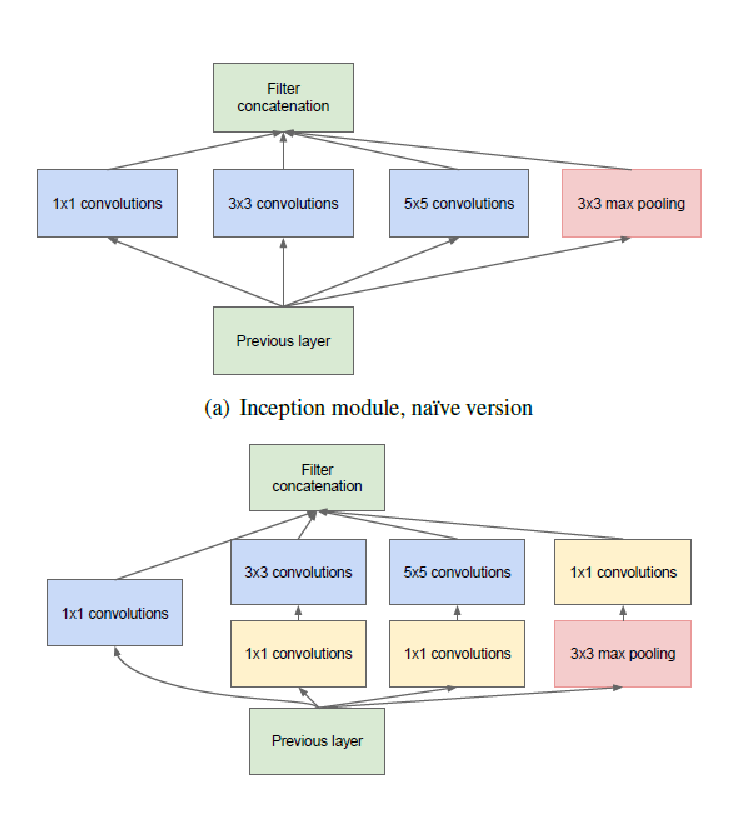
\includegraphics{GoogLeNetModule.eps}
  \caption{GoogLeNet Module}
  \label{fig:4.1}
\end{figure}The network set-up provided by SSD is built using the deep-learning framework Caffe, so its functions are intimately involved in the final project.
Caffe allows for command line instructions to be sent to define the network.
To set up the network and Caffe properly we are using the tools provided by Caffe itself and the components found in the SSD branch of the main Caffe repository on Github.
\newline
\newline
Training of the neural network will be done on NVIDIA GPUs on the Amazon Web Services cloud as well as on normal PC's.
Cloud computing is mostly used in the later stages to speed up the training process.
Once the network is fully trained, it will be deployed on the Jetson to play the game Galaga in real time.
\newline
\newline
The structural goal of the neural net changes between two stages.
In the first stage, the structure of the neural net is meant purely to teach it how to recognize and categorize in game objects from images.
In the second stage, the neural network will be deployed on the Jetson TX1 and will take active game information.
It will use that information to make one of four choices: move left, move right, stop, or shoot.
More detail on the training will be given in section \ref{sssec:num2}.

\section{Information viewpoint}\label{sssec:num2}%Luay

The data in this section consists of image processing of the game being played as well as the trained neural network.
This section will go in depth of both how image processing will be done as well as different ways to train and improve the neural network.
A pseudocode will be included to give an overview of where these data will be used in this project.
Also, the pseudocode in \ref{sssec:num3} will include a general algorithm to show how output decision's layer works.

\subsection{Set up image dataset}%Luay

Setting up image set for training and testing requires using annotation methods that can be used to label and identify objects from any given image.
In this project, Pascal VOC annotation is being used because it's the most common and supported by the majority of deep learning frameworks as well as neural networks.
The deep learning framework we are currently using supports Pascal VOC and Coco but only Pascal VOC is being used.
However, in order to prepare the annotations we would need to separate train validation images and test images so we can easily list them in a text file along with their path and XML which is the annotation file.
In addition, we would need to write down a label map file that lists all the objects that need to be identified by the neural network.
Overall, the files are needed in order to create the LMDB database are trainval.txt, test_name_size.txt, test.txt, lebelmap_voc.prototxt.
Examples of how to write those files are in \ref{sssec:num33}.
\subsection{Neural training methods}%Gabe

The training of the neural network will be done in two stages.
In the first stage, we will be using images created from the game to teach the network how to recognize in game objects.
Given that GoogLeNet was designed with image categorization in mind, this set-up will be easy to create and bring to functionality.
We will feed the network with images doctored by OpenCV and it will interpret them and label them.
Once it has a high degree of success in correctly identifying in game objects, we will take the training to stage two.
\newline
\newline
In the second stage of training we will be feeding the network images directly from live game progress.
The game will be running and the network will be deployed on the Jetson.
The network will be given the ability to take actions based on the objects it identifies on screen.
Positive feedback will be given to the neural network when it correctly kills an enemy or completes a level.
Negative feedback will be given to the network when it dies, gets a game over, or loops too long doing nothing.
As the neural network plays the game, it will improve performance and eventually be considered proficient.

\subsection{Input image processing}%Luay

After having a trained neural network, a software written in python will start by loading the necessary dependencies, which are OpenCV.
Then, a video capture of the game will take a place to record the monitor where the game is being played using OpenCV's API.
The hardware connection of the camera, as well as the control mechanism of the game, shall be explained in section \ref{sssec:num1}.
Since videos are just consecutive images, OpenCV will be used to get each frame and then pass the image to the input of neural network.
Then we would need to do a forward call to the network's API using Caffe which give us the output from the neural network.

\subsection{Data visualization}%Chris

It was necessary to figure out how to display the results of each round.
We decided it would be best to have a summary, graphical display of the data at the end of the playthrough.
Once the program runs out of lives, a screen will appear, graphing statistics about the machine's performance.
These statistics will include things such as how long the machine lasted, how many levels it completed, which enemies or objects took away the most lives, and so on.
Having detailed and easily readable data is key to knowing how to train the machine to keep performing better in the game.


\newpage

\subsection{Setup Image Data Sets Example}\label{sssec:num33}

\subsubsection{trainval.txt}
train/image1.png train/image1.xml

\subsubsection{test.txt}
test/test1.png test/test1.xml

\subsubsection{test_name_size.txt}
imageName imageWidth imageHeight\newline
test1     1080       1920

\subsubsection{labelmap_voc.prototxt}
\{\newline
name:"player",\newline
label: 0,\newline
display_name:"player"\newline
\}\newline
\textbf{Note:} Label is a numerical value and should be incremented every time a new label is added.

\subsection{Pseudocode}\label{sssec:num3}
% \subsection{Decision Layer Pseudocode}\label{sssec:num300}
\begin{algorithm}
  % Load necessary packages for openCV, and Caffe.\.
  % Load the trained net.\.
  % Convert the trained net to an object which OpenCV understands.
  % Start video capture.
  % For each frame in the video capture:
  \emph{Reshape the Layer to set output one thing of size 1 - for possible outputs such as left,right,shoot}\;
  \emph{In Forward Function:};\newline
  \nl$player_x,player_y\leftarrow Coordinates Of the label Player$\;
  \nl$topData\leftarrow buttom[0]->date()$\;
  \ForEach{object on the game}{
    \If { (object.y $\geq$ 300) and and (object.x $\leq$  player_x+200) }
    {
      \nl$topData[0]\leftarrow 0$\;
    }
    \ElseIf{ (object.y $\geq$ 300) and (object.x $\leq$  player_x+200) }
    {
      \nl$topData[0]\leftarrow 1$\;
    }
    \ElseIf{ (object.x $\leq$  player_x+100) and (object.x $\geq$  player_x-100) }
    {
      \nl$topData[0]\leftarrow 2$\;
    }
  }

    \caption{Decision Layer}
\end{algorithm}

\begin{algorithm}
  % Load necessary packages for openCV, and Caffe.\.
  % Load the trained net.\.
  % Convert the trained net to an object which OpenCV understands.
  % Start video capture.
  % For each frame in the video capture:
  \emph{Load necessary packages for openCV, and Caffe}\;
  \emph{Load the trained net and label map}\;
  \emph{Do input preprocessing using Caffe Transformer API}\;
  \emph{Start video capture}\;
  \ForEach{frame in the video capture}{
    \emph{Load the frame to data layer which is the input of the nerual network}\;
    \emph{Call Caffe forward API to get decision output from the network}\;
    \emph{Send the decision through the network to the game hosted computer with a command such as left, right and shoot}\;
  }

    \caption{Jetson TX1 plays Galaga}
\end{algorithm}

\section{Interaction Viewpoint}\label{sssec:num1}%Chris

This section details how our physical hardware components interact to form a cohesive system.
It will outline several pieces of hardware used to realize the goal of playing galaga.

\subsection{Hardware setup}%Chris

While working with the Jetson TX1 there are several things that we needed to decide.
These included our methods to communicate with our client, and the hardware used with the Jetson.
Choosing out hardware was key to determining how each piece would fit into the design.
\newline
\newline
Our project will actually need to be able to control the game.
Inputs from the neural net need to be received by the game so that it can be played.
To do this we decided not to use the standard keyboard.
Using a keyboard requires a lot of additional coding to map the Jetson to the controls.
We had originally decided that we would use a gaming controller and wire the Jetson to it so that the neural net could send the game commands.
A game controller would have significantly reduced the work load because it would have already contained a lot of built in functionality that we needed to connect it to the Jetson.
However instead of requiring another piece of hardware we decided to just use Windows APIs and a client server system.
The Jetson will be able to send commands to the game through an ethernet cable.
This setup is outlined in figure \ref{fig:4.2}.
\newline
\newline
\begin{figure}
  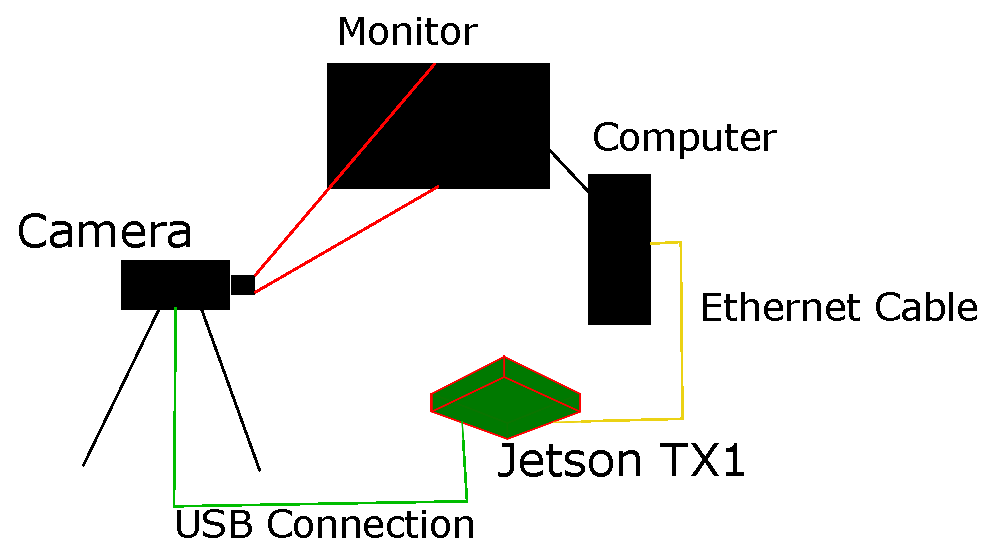
\includegraphics[width=\textwidth]{design.eps}
  \caption{Hardware Layout}
  \label{fig:4.2}
\end{figure}% Figure \ref{fig:4.3} shows the basic layout.
Since the Jetson has to learn how to play the game on its own it needs to be able to see the game.
By see I mean that video has to be captured and translated into data the neural net can understand.
We were able to buy a pretty inexpensive camera that could capture more than enough detail.
It only cost about \$25.
This option had not been in the tech review originally but after some work on the project we realized that in order for the neural net to play the game it didn't need incredibly high quality images.
The neural net only needed images where it was obvious to see what enemies were being recorded.
Also to react to the game quickly enough to beat the first level we realized the neural net wouldn't have to process more than 30 frames per second.
The camera will be connected to the Jetson and aimed at the monitor, which is connected to the computer running the game.
The program will first be trained by being given the video input to recognize and characterize objects within the game.
We will set up tables so that the neural net will be able to store information such as the locations of objects.
Once the objects and tables are set up the neural net will be able to train itself by playing the game, sending commands through an ethernet cable.
Its decisions will be based on the table of information that it stores and will increasingly be able to survive the game longer.
Eventually the neural net will learn to respond to certain patterns in the table in order to become better at the game.

\section{Conclusion}
The goal of this design document is to provide the how to of this deep learning project which will be turned to the NVIDIA's deep learning institute to use it in a deep learning course.
The overall steps for this document are to teach the Jetson TX1 to play the game Galaga by training a neural network to identify game objects and become effectively able to move the player away from enemies.
This can be done based on three major phases which are preparing images for the game objects, training a neural network based on the set of images with labels, and finally by using a camera connected to the Jetson TX1 while the game hosted on a different machine that is being controlled using the Jetson TX1 and a controller input.

\end{document}


\section{Changes made from the design document}
Several things outlined in the design document's original form were far off base from the reality of the finished product, as is to be expected.
When the original design document was written, our team had not fully researched the topic and we were still learning how to go about accomplishing the task. 
The first major change from initial design was the choice of neural network architecture. 
Originally we had planned to use a model based on GoogLeNet to accomplish the task.
As our research expanded outward, we discovered SSD, which allowed us to not only detect the presence of objects in a screenshot, but also to identify where they were.
We also ended up changing the structure of the decision output.
While initially we had intended to build a set of custom learning logic so the neural network could learn to make the game decisions on its own.
Due to the difficulty of this relative to the time we had, we scaled back to one layer of in-built decision logic.
\newline\newline
When it came to our training methods we also had to re-examine our initial approach.
We set up our images in largely the same way as described, but not with any doctoring through OpenCV.
We did still do stage one of training, using labelled images to train the network to recognize specific objects.
Due to the above changes, training stage two was dropped entirely.
There was no longer a component of our project to train as described in stage two.
We also did not use any kind of cloud computing for the training, as our own computers proved sufficient.
\newline\newline
We never implemented any kind of automatic data visualization for output of the neural network.
We did still use a client server system to allow the neural network to communicate with the computer hosting the game.
The client-server code was ultimately coded in Node.js.
The final hardware layout was pretty much exactly as described, though it could be adapted to use wireless communication and the inbuilt camera on the Jetson TX1.

%\section{Technology review}

%%Copyright 2014 Jean-Philippe Eisenbarth
%This program is free software: you can
%redistribute it and/or modify it under the terms of the GNU General Public
%License as published by the Free Software Foundation, either version 3 of the
%License, or (at your option) any later version.
%This program is distributed in the hope that it will be useful,but WITHOUT ANY
%WARRANTY; without even the implied warranty of MERCHANTABILITY or FITNESS FOR A
%PARTICULAR PURPOSE. See the GNU General Public License for more details.
%You should have received a copy of the GNU General Public License along with
%this program.  If not, see <http://www.gnu.org/licenses/>.

%Based on the code of Yiannis Lazarides
%http://tex.stackexchange.com/questions/42602/software-requirements-specification-with-latex
%http://tex.stackexchange.com/users/963/yiannis-lazarides
%Also based on the template of Karl E. Wiegers
%http://www.se.rit.edu/~emad/teaching/slides/srs_template_sep14.pdf
%http://karlwiegers.com
% \documentclass[letterpaper,10pt]{article}
\documentclass{scrreprt}
\usepackage{listings}
\usepackage{underscore}
\usepackage[bookmarks=true]{hyperref}
\usepackage[utf8]{inputenc}
\usepackage[english]{babel}
\usepackage{graphicx}
\usepackage{amssymb}
\usepackage{amsmath}
\usepackage{amsthm}

\usepackage{alltt}
\usepackage{float}
\usepackage{color}
\usepackage{url}

\usepackage{enumitem}

\usepackage{geometry}

\usepackage{titling}
\usepackage{rotating}
\usepackage{pgfgantt}
\usepackage{xcolor}
\usepackage{anyfontsize}

\usepackage{tabularx}
\newcommand{\tabitem}{~~\llap{\textbullet}~~}

\ganttset{group/.append style={orange},
milestone/.append style={red},
progress label node anchor/.append style={text=red}}

\geometry{textheight=8.5in, textwidth=6in}
\hypersetup{
    bookmarks=false,    % show bookmarks bar?
    pdftitle={Software Requirement Specification},    % title
    pdfauthor={Jean-Philippe Eisenbarth},                     % author
    pdfsubject={TeX and LaTeX},                        % subject of the document
    pdfkeywords={TeX, LaTeX, graphics, images}, % list of keywords
    colorlinks=true,       % false: boxed links; true: colored links
    linkcolor=blue,       % color of internal links
    citecolor=black,       % color of links to bibliography
    filecolor=black,        % color of file links
    urlcolor=purple,        % color of external links
    linktoc=page            % only page is linked
}%
\def\myversion{1.0}
\date{}
%\title
\usepackage{hyperref}
\begin{document}

\begin{flushright}
    \rule{16cm}{5pt}\vskip1cm
    \begin{bfseries}
        \Huge{Technology Review and Implementation Plan}\\
        \vspace{1.9cm}
        for\\
        \vspace{1.9cm}
        Deep Learning on Embedded Platform\\
        \vspace{1.9cm}
        \LARGE{Version \myversion}\\
        \vspace{1.9cm}
        Prepared by Christopher Johnson, Luay Alshawi, Gabe Morey\\
        \vspace{1.9cm}
        CS 461 Fall Term\\
        \vspace{1.9cm}
        \today\\
    \end{bfseries}
\end{flushright}


\chapter{Abstract}
Working on a large scale project requires multiple pieces to come together in the right way. If the right pieces aren’t used,
the project will turn out poorly for it. In this document we lay out several different components necessary to build our project,
which consists of building a neural network setup which can learn to play the game Galaga.
We will discuss different technologies that can be used to satisfy the needs of those components and come to a conclusion on which technologies to use.
 This document also lays out which team members are responsible for different pieces of the final project.

\chapter{Duties}
\section{section name}
\subsection{Gabe Morey}
I will be in charge of setting up the neural network for learning on the embedded processor. It is
my job to make sure the network can be properly trained and utilized to play the game Galaga.
With this in mind, i will be reviewing the different deep learning frameworks around the web
and deciding on one to use for the project. I will also be in charge of the actual neural network
we train and will be covering several established networks. I will also be reviewing several
clouds that allow for GPU use without physically having a strong enough GPU for neural
network training. So in total I am responsible for making sure we have a proper neural network
structure which has ample cloud based processing power to perform the task we have set out for
it.

\subsection{Luay Alshawi}
I will be responsible for setting up the operating system development environment. 
I will make sure that all the requirements development dependencies such as visual libraries, programming languages, and neural network work on the Linux operating system. 
Also, I will be responsible for making sure the visual library is working and can capture the game Galaga then feed it to the neural network. 
Although we as developers we should not be struggling with the programming language but I will be responsible for making sure we are using the right programming language and works on Linux.

\chapter{Technologies}
\section{Visual Library}
\subsection{Open CV}
An OpenCV (Open Source Computer Vision) is a library that can be used with tons of different languages(C, C++, Java, Python, etc.).
 It provides standard things such as image capture, Faces recognition, Gesture recognition, Motion tracking, Mobile robotics, Object identification and Image manipulation.
 OpenCV was built to provide a common infrastructure for computer vision applications and to accelerate the use of machine perception in the commercial products.
 Being a BSD-licensed product, OpenCV makes it easy for businesses to utilize and modify the code (Team).
\subsection{SimpleCV}
SimpleCV is a framework including several libraries and uses Python for scripting.
Due to the nature of python, it can either run scripts or use an interactive shell to do computer vision computation and related tasks.
With it, you get access to several high-powered computer vision libraries such as OpenCV – without having to first learn about bit depths,
file formats, color spaces, buffer management, eigenvalues, or matrix versus bitmap storage (Sight Machine, Inc).
\subsection{Community Core Vision}
CCV (Community Core Vision) library is an open source/cross-platform solution for blob tracking with computer vision.
Supports a wide range of camera devices with the ability to stitch and switch in between sensors on the fly.
It is built on C++ for real-time performance and stability using common frameworks including OpenCV and open Frameworks.
To minimize the code base, it gives up non-essential functionalities aggressively.
It is not a library for you to experiment different algorithms.
It is a library for you to use in your applications (LiuLiu, 2012).

\subsection{Goals}
Computer vision library is used in order to teach a computer machine to learn from video and images in order to understand real-world feel by detecting,
classifying and identifying objects and events.
In real world application, an example is the BMW parking assistant and NASA used this to land the Mars Rover.
It is also used in industries where it is referred to as machine vision, where information is extracted for purposes of supporting a manufacturing process.
A good example is a quality control where details of final products are being automatically inspected in order to find defects.
Computer vision aids in machine learning giving computers the ability to learn without being programmed,
construction of this algorithms helps a computer learn and make predictions on data,
this helps in overcoming strict static program instructions by making data-driven predictions or decisions,
through building a model from sample inputs.
Thus, computer vision library is needed to make sense of images and teach a computer to play the game Galaga.

\subsection{subsection name}

\subsection{Comparision Table}
\begin{center}
  \begin{tabular}{| l | c | r |}
    \hline
    Open CV & SimpleCV & Community Core Vision \\ \hline
    \parbox{5cm}{- Libraries for most other languages(C,C++ and Python)} & \parbox{5cm}{- Interactive shell for testing} & \parbox{5cm}{- Uses statically-linked library} \\
    \parbox{5cm}{- Great for large scale programs} & \parbox{5cm}{- Great for quick demonstration purposes} & \parbox{5cm}{- Gives up non-essential functionalities aggressively} \\
    \parbox{5cm}{- OpenCV is best for implementation as it offers a lot more possibilities} & \parbox{5cm}{- Works very well with Pythons} & \parbox{5cm}{- It is not a library for you to experiment different algorithms} \\
    \hline
  \end{tabular}
\end{center}

\subsection{Discussion}
OpenCV is open source, free for commercial and research use under the BSD license.
It is also cross-platform from, and runs on Windows, Linux, Mac OS X, mobile Android and iOS. With SimpleCV, you get access to several high-powered computer vision libraries such as OpenCV- without having to first learn about bit depths, file formats, color spaces, buffer management, eigenvalues, or matrix versus bitmap storage.
SimpleCV is free to use, and because it is open source, you can also modify the code if you choose to.
It’s written in Python, and runs on Mac, Windows, and Ubuntu Linux and is also under the BSD license.
CCV is an open source/cross-platform solution for blob with computer vision,
it is published under an open-source LGPL license on Github to allow for others to contribute features and forks.


\subsection{Best Option}
CCV is a library for small applications.
For quick prototyping SimpleCV is far superior, but for actual implementation/usage OpenCV offers a lot more possibilities.

\section{Devolopment Operating System}

\subsection{Windows}
Windows OS, computer operating system (OS) developed by Microsoft Corporation to run personal
computers (PCs). Featuring the first graphical user interface (GUI) for IBM-compatible PCs, the Windows
OS soon dominated the PC market (Britannica, 2015). Microsoft Windows operating system was
developed by Microsoft to overcome the limitation of its own MS-DOS operating system.

\subsection{MAC OS}
The Mac OS or Mac OS is a series of graphical user interface-based operating systems developed by
Apple Inc. for their Macintosh line of computer systems (Dong, 2007). Mac Os was designed only to run
on Apple Computers. In 1984, Apple introduced the Macintosh PC with the Macintosh Operating
System. Apple names its OS as “Mac OS”, beginning in 19997 which previously known as “System”.

\subsection{Linux}
Linux is an open source operating system, or Linux OS, is a freely distributable, cross-platform operating
system based on Unix that can be installed on PCs, laptops, netbooks, mobile and tablet devices, video
game consoles, servers, supercomputers and more (Beal). Linux is a Unix-like, Kernel-based, fully
memory-protected, multitasking operating system.

\subsection{Goals}
Operating system will be used as the host environment for the deep learning project.
It will be used to run the software of the image visualization as well as the neural network.

\subsection{Criteria}
Mac OS is a two layered system: the “attractive GUI” sits atop Unix core, and Unix is best-known for its
security features. It’s simply impossible to install a destructive Trojan or virus unless the user explicitly
allows it root access via typing in the admin password. Mac OS’s built-in firewall is set up to work
unobtrusively out of the box as well as being highly configurable. Mac OS is incredibly stable. Apple
controls production from start to finish, so every part of a Mac is designed and tested to work together.\newline


A Microsoft window is easy to use as compared to other operating systems. Windows gives you an
advantage of checking the performance of your PC. No need to install drivers of any peripheral devices.
It is a windows operating system meaning every task is performed in its own window. Because of its
wide use it has documentations and tutorials available to learn the OS. Windows offers support to the
user as it has its own help section, and websites/forums where you can talk to people and gain
information about Windows. There are also books available for each version of windows to help you.
Windows has an administrative user that can make changes to the computer, but it has other users that
can perform small tasks. You need the administrator’s password to change anything if on another user.
\newline
Linux is a source operating system. Any programmer can modify it due to its needs. It is a free software
that anyone can download it from web and install it on its PC. Many PC users can install Linux to its
system there is no specific requirements for installing it. Linux has books for help and also online forums.
Linux security requires a user to enter an administrator’s password in order to make changes or
download things, so it is harder for harmful programs to gain access to the computer.

\subsection{Comparision Table}

% \begin{table}[]
% \centering
% \begin{tabular}{|l|l|l|l|l|l|l|l|}
% \hline
% Operating Systems & Security                                                                                              & Price                                 & Compatibility                                                                                              & Reliability                                                                             & Package Manager                                                                                   \\ \hline
% Windows OS        & \parbox{5cm}{There are many types of viruses in Windows OS because of a large amount of market share}               & Windows is less expensive than Mac OS & Anyone can install any type of game into Windows PC,as it is,compatible to all types of software and games & Windows is very reliable but due to its affinity to viruses it,struck                   & No official package manager                                                                         \\ \hline
% Linux OS          & \parbox{5cm}{There are lesser amount of viruses in Linux as compared to,Windows because Linux is an open source OS & Linux software is totally free}        & Since Linux is an open source software you can program the,software that you want.                         & Since Linux is not a complete OS you can modify it for that,type of usage that you want & Most Linux distributions provide official package manager,software to install third party software \\ \hline
% MAC OS            & \parbox{5cm}{There are no virus in Mac OS because you can install Mac only,on Apple devices}      & Apple devices are too much expensive  & Most software are not compatible with Mac OS so you feel,limited on Mac OS                                 & Mac is very reliable and smooth because it has no viruses that,drag its performance     & No official package manager                                                                        \\ \hline
% \end{tabular}
% \end{table}
\subsection{Discussion}
Though some operating systems like Linux may seem the better option because of its flexibility to be
used in any kind of way, the choice is usually up to the user. If you’re a gamer, then you have no choice,
go for Windows. Software Developers might prefer Linux and video/graphics producers will probably
tend towards Mac.

\subsection{subsection name}
After all is said and done, Linux eventually comes out as the winner. The reason Linux to be the better
option is because it is powerful, runs on multiple hardware platforms. Users like its speed and stability,
has no requirements for latest hardware. It is also free and licensed under GPL. Also vendors aredistributors who can package Linux. The ease to install software as it is also useful for software
development purposes.


\section{Programming Languages}

\subsection{Python}
Python which is an interpreted, objected – oriented language which is similar to PERL as it has a high-
level built in data structures with a dynamic binding making it attractive for a rapid application
development since it is a scripted language for connection of existing components. These creates
readable and hence reducing the cost of development and maintenance.

\subsection{C++}
C++ has classes which used in the form of an objective where it combines data representation as while
as methods employed in the manipulation of the data in a neat package this include arithmetic, bit
manipulation, logical operation.

\subsection{Java}
As for the Java this is a programming language which helps in creating applications that may run on a
single computer Or other server in a network as the portable as it is fast, secure and most reliable and it
is easier to learn however one should note that Java software cannot be installed alone hence a plugin
software is needed.

\subsection{Goals}
The basic knowledge in programming is such a critique in that it has captured the most significant arc of
human life. Slowly computer and software are taking the functions which affect our lives and has
become an inescapable part of our life. In the modern world software products are used in selection
form for the technique which improves the quality of the product of the software development. Today
software is accurate, faster and cost effective in our today life in educational, professional as well as
personal.

Choosing a programming language depends on the client, the need it solving, this happens in designing
whereby the designer indicates guidance to the architecture of the project in detail on the system
especially activities involved in designing, development, and enhancement as well as maintenance of the
software. In the design phase, a specific system should be produced which gives necessary requirements
hence ensuring maximum ease of use and effectiveness in the documentation where retrieval of
information is crucial hence minimizing time as while as effort and more so the development cost. Since
it involves carrying out a community consensus enhancing a significant number of people in working
together in achieving a common goal. Thus, picking a programming language can bring ease of
development as well as productivity to the project outcome.

\subsection{Criteria}
The criteria’s for picking the right programming language depends on many important factors. The fist
factor to consider is the documentation because as a developer well-written documentation is the best
source for finding resources, explanation and language features. The second factor is the community,the larger the community the better since help can be found easily on the internet and an example of
that is stackoverflow.com. The third factor is the ease of execution which measures the steps for a
software to execute and run. The fourth factor is used to measure the requirements for a programming
language to run on an operating system. The fifth factor measures the standard libraries and data
structures that come with the programming language by default. The last factor measures the codes
density which compares the line of codes required to do certain tasks.

\subsection{Comparision Table}
\begin{center}
  \begin{tabular}{| l | c | r |}
    \hline
    Open CV & SimpleCV & Community Core Vision \\ \hline
    \parbox{5cm}{- Libraries for most other languages(C,C++ and Python)} & \parbox{5cm}{- Interactive shell for testing} & \parbox{5cm}{- Uses statically-linked library} \\
    \parbox{5cm}{- Great for large scale programs} & \parbox{5cm}{- Great for quick demonstration purposes} & \parbox{5cm}{- Gives up non-essential functionalities aggressively} \\
    \parbox{5cm}{- OpenCV is best for implementation as it offers a lot more possibilities} & \parbox{5cm}{- Works very well with Pythons} & \parbox{5cm}{- It is not a library for you to experiment different algorithms} \\
    \hline
  \end{tabular}
\end{center}

\subsection{Discussion}
All three programming languages have the same level of power based on the comparison table.

\subsection{Best Option}
Python is a great option for our project since it needs less step to run compare to the other
programming languages. Also, python comes with wide variety of libraries and data structures such as
arrays, dictionaries, and tuples.


\section{Deep Learning Framework}

\subsection{Theano}
Theano is a library for Python which focuses on simplifying and speeding up the calculation of
complex mathematical expressions that use multidimensional arrays. It was originally created by
LISA lab for use in quick development of machine learning algorithms. It uses its own compiler
and functions as an extension to the Python programming language. Its optimizations allow for
the translation of commands to GPU and CPU instruction code for increased speed of operation.
Theano can perform graph optimizations and compile parts or all of a graph into CPU or GPU
instructions [1]. It also has the ability to detect certain unstable expressions and replace them
with much more stable algorithms for the program run. It supports tensors and sparse type
operations. Theano provides many more functions related to graph evaluation and mathematical
optimization. Theano is still in development and is currently at version 0.8 [1]. This technology
is primarily useful in deep learning for its ability to interact directly with a GPU and process
graph data. This allows for the deep learning algorithms made with it to process data at high
speeds, though I have not found any solid metrics of how fast it can process a graph. The speed
does depend on the quality of the GPU used and the nature of the graph being processed.

\subsection{Caffe}
Developed by the Berkely Vision and Learning Center, Caffe is designed specifically as a
framework for deep learning. According to their website, it was made with “expression, speed,
and modularity in mind,” [2]. Caffe can interface with Python and Matlab, but its primary
interface is command line. It uses its own schema to define layers in its deep learning network.
Caffe uses what its developers call Blobs, which are essentially multidimensional arrays that
wrap the data that will be processed or sent along by Caffe. Blobs are used to “conceal the
computational and mental overhead of mixed CPU/GPU operation by synchronizing from the
CPU host to the GPU device as needed,” [2]. It can allocate memory as needed for its operation.
The site claims they believe their program to be convnet implementation possible, though their
metric of speed is applied to one specific GPU [2]. The system supports optimizations for many
different data operations required for interfacing with a neural network and training it properly.

\subsection{Torch}
Torch is a computing framework that uses LuaJIT as its main code language interface. It has
“support for machine learning algorithms that put GPU’s first,” [3]. Torch supports several
models and functions necessary for scientific calculations such as linear algebra routines,
numeric optimization, GPU support, n-dimensional arrays, indexing, slicing, and transposing
among others [3]. Torch’s Lua base provides is with incredible speed as compared to other
programming languages, but this comes with the downside of less cross-compatibility. Lua is not
a widely used programming language, so support for it is less common than support for the bases
of many other frameworks programmed in langauges like C, C++, and Python [5]. Torch
provides tensor support and packages for machine learning and computer vision [4]. The GPU
focus of torch makes it ideal for GPU based neural network training.

\subsection{Choice of Framework}

This project will be using Caffe. Caffe has widespread support for systems and has been around
long enough to have plenty of documentation on its use as well as examples of it in action. Caffe
is coded at base in C++, which makes it easy to set up on most systems. The python framework
provides support for an easy to use language that everyone in the group understands and can
utilize to full potential. The systems integration with major neural nets is well documented as
well.

\section{Neural Network}

\subsection{Information}
Regardless of which neural net being discussed, a few things need to be laid out to clarify what
we mean by neural network and other terms related. A neural network is essentially a
complicated decision graph built in layers by a machine learning algorithm. Each node is
referred to as a neuron and has its own learned weights and bias. A convolutional neural network
assumes all of its inputs are images, thus reducing the parameters for its use [13]. Because our
project relies on visual input from a video game, we can process all incoming data as images.
This section will cover the different convolutional models we could use to process our data.

\subsection{GoogLeNet}
GoogLeNet is a neural network design which uses Inception architecture. The Inception
architecture is designed “to consider how an optimal local sparse structure of a convolutional
vision network can be approximated and covered by readily available dense components,” [10].
The idea behind this lies in how it deals with the layers that make up a neural network. It
attempts to cluster these layers in optimal arrangements for program flow. It also attempts to
reduce dimensionality of the network whenever computational requirements would get too high.
The chief goal of the architecture is computational efficiency and practicality [10]. GoogLeNet is
22 layers deep. It uses about 100 layers to actual construct this network, though the exact number
is reliant upon how many layers are actually counted by the machine learning infrastructure [10].
The document covering GoogLeNet contains a rough estimate that, given the dataset used for its
premier competition, the network could be trained to convergence using a high-end GPUs within
a week. The biggest limitation of training speed is memory usage [10].

\subsection{AlexNet}
AlexNet is a neural network architecture designed by Alex Krizhevsky, Ilya Sutskever, and
Geoffrey Hinton at the University of Toronto. It was trained originally with a dataset of “over 15
million labeled high-resolution images belonging to roughly 22,000 categories,” [11]. The
architecture contains eight learned layers; five of these layers are convolutional and the other
three are fully connected [11]. The architecture is designed to be slit across two GPUs, with each
GPU running separate layers. The GPU’s only communicate between each other on specific
layers. The convolutional layers filter the image size for proper processing. The network has 60
million parameters each fully connected layer has 4,096 neurons [11]. The architecture uses two
forms of data augmentation to ensure that the images are processed properly despite filtering size
down. The aim is to reduce complexity of calculation and increase speed. The first method
consists of image translations and horizontal reflections, while the second consists of altering
intensities of RGB (Red Green Blue) channels in the images used to train the network [11]. This
network achieved a test error rate of 15.3\% in the ILSVRC-2012 neural network training
competition, placing it among the top 5 entrants.

\subsection{OxfordNet}
OxforNet is a neural network architecture designed by Karen Simonyan and Andrew Zisserman
at the University of Oxford. One of the key features of this architecture is that all of the filters
used in the convolution layers for image processing are quite small. Most other convolutional
neural networks work down from slightly larger filters, but OxfordNet remains steadier in its
filter size. It makes up for the lost image depth through having 16-19 weight layers in the
network [12]. The training methods of this network are similar to those used for AlexNet, as this
framework was built to improve upon that architecture. The weights of the node layers at
initialization plays a key role in affecting how long it takes the net to learn properly [12]. The
structure requires multiple GPUs to practice parallelism in its data processing. The network on
its own achieved a 7.3\% test error rate, and when two models were combined the error rate was
only 6.8\%.


\subsection{Choice of Network}
After reviewing the documentation, implementations, and performance of the neural network
architectures available, we decided to use GoogLeNet. GoogLeNet is a newer architecture and
provides heavy processing power for multiple images. It takes advantage of the most nodes while
also having a solid plan to compress its data usage, which results in the kind of speed we need
for real-time image processing. Our network needs to be able to process the game fast enough to
play, and GoogLeNet offers a viable model for doing so.

\section{GPU Cloud}
\subsection{EC2}
EC2 is a cloud computing environment set up by Amazon Web Services. The EC2 cloud
supports a wide array of practical features for computing on a large scale. The system supports
high performance computing with many more cores than the average CPU. The cloud provides
“up to 16 NVIDIA K80 GPUs, with a combined 192 GB of GPU memory, 40 thousand parallel
processing cores, 70 teraflops of single precision floating point performance, and over 23
teraflops of double precision floating point performance,” [6]. The GPUs are capable of
supporting CUDA and OpenCL frameworks. Machine learning is specifically listed as a taskwhich these GPU’s are able to support, which makes it a good fit for a deep learning project. The
high GPU count also allows for high real time graphics processing, which pairs well with things
that require graphical input. The cloud supports many more features such as security,
networking, and auto scaling, but the high GPU count is the most impactful to its use on this
project. Pricing for on demand use varies per server and memory needs from less than a dollar
per hour to around \$17/hour.

\subsection{Nimbix}
Nimbix is a cloud computing and storage company. Their cloud supports several different types
of NVIDIA GPUs, including the K40 and K80. The cloud supports OpenGL, OpenCL, and
CUDA environments [7]. The cloud offers up to 128 GB of RAM and 1 Terabyte of storage. The
JARVICE platform on their cloud offers support for big data and heavy computation. It contains
an API for use specifically with GPU’s. It uses custom Linux systems, referred to as Nimbix
Application Environments, to build and run application on the cloud [8]. The environments have
full access to the CPU, GPU capacity, and memory of the underlying hardware. Nimbix offers
pay rates for up to 16 cores and up to two NVIDIA Tesla K80 or K40 GPUs. The price of using
two K80s hits \$5.00/hour. The Nimbix cloud has a lot of articles and documentation surrounded
its uses in high power computing and deep learning.

\subsection{Cogeco Peer 1}
Cogeco Peer 1’s cloud offers customized GPU server solutions with NVIDIA Tesla series GPUs
[9]. Cogeco Peer 1 does not offer on-demand server use. To use their cloud, one must rent a
physical dedicated server from them. They provide setup and management for the cloud server.
They tailor GPU solutions to the tenant’s needs. They can set up the server with several
operating systems including Windows and Red Hat. Their website promises rapid response to
any server issues experienced while using their product. The customizability of the setup offers a
concrete way to ensure the cloud has the proper setup for our group needs, but requires much
more setup time. The company seems to largely focus on business solutions rather than
individual use, so it’s not very well suited to our project needs.

\subsection{Choice of Cloud}
Given the information we have on cloud computing systems, we have chosen to use Amazon
Web Services EC2 due to its convenient use, high availability of powerful GPU processing, and
support for frameworks we’ll be working with. Furthermore, our client has offered to handle the
costs of this cloud computing platform, which means that we will not need to pay out of pocket
to use its services. Nimbex is a very tempting second, as it offers very good pricing and a lot of
NVIDIA GPU support for Neural Network training. However it isn’t quite as powerful as the
Amazon cloud. Cogeco Peer 1 is much too focused for long term business solutions to be a
reasonable option on this project. It also offers less power than the Amazon cloud.

\section{Jetson...}

The role of making sure everything runs smoothly on the platform required of us to implement out solution on can be devided into three categories.
These categories are finding the right communication methods with our client for group meetings, deciding what camera technology we need, and figuring out the best way to visialize the data.
For each of these three tasks I have found three approaches that I have research and given thorough consideration.
This is to ensure that we are making the best possible decisions when working with the Jetson TX1.

One of the most omportant aspects of a group project is communication.
This is especially true when we're working with a client who has tasked us with using a certain platform.
There will most likely be many times when we'll need to discuss something about the Jetson.
There are many very popular and suitable tools available to conduct online meetings.
These include Skype, Discord, and Team Speak.
Skype was founded in 2003 by Niklas Zennström.
Skype has a lot of features that Discord and Team Speak don't have.
One of these features includes screen sharing.
This feature could be very beneficial during group meetings when a group member has to explain something visually.
Our group has used Skype twice in the past and the sound quality was good enough for everyone to understand each other.
Discord and Team Speak also do not allow video calls, they only provide groups to voice and text chat.
One down side with Skype however is the presence of bugs.
Among reviewers, skype is the least reliable.
A huge factor in our decision on with communication tool to use is what everyone is comfortable using.
Since most people are alread familiar with skype and our group has alread conducted two meetings with it, skype might be the best tool for the job.

Discord, which is the most recent VoIP service released, is known for its very nice user interface.
This service also does not require a download.
Users can log on and join a Discord server using their browser.
Discord hosts its own servers which are very reliable.
Joining a call is very simple.
Whoever is hosting the server simply sends each group member a link.
Other group members simply click the link and join the voice server using either their web browser or downloaded application.
It also has a very good chat system.
Call quality is not limited to a group members poor internet.
Discord is also very light weight and puts much less strain on the cpu than Skype and Team Speak.
However, Discord does not have many of the Skype features including video calling and screen sharing.

Team Speak is best known for its sound quality.
Team Speak is the second oldest voice chat service, which has been in development since 2004.
The newest version is Team Speak 3.
Team Speak has the greatest sound quality and reliability out of all three VoIP applications.
One of the big problems with Team Speak however is its user interface.
For beginner users it can be a lot more difficult to figure out.
Many reviewers say that it has the worst user interface design compared to Discord and Skype.
This is probably a product of its customizability.
There are many ways to improve a users experience with Team Speak including downloading user interface package downloads.
If there are only a couple of us in the group already familiar with how to use Team Speak then it probably isn't the best choice.
However, if everyone is alread accustomed to using Team Speak then our group might be able to benefit from Team Speak's greater flexibility.

For deciding what kind of camera we should use, there are a lot of factors to consider.
The camera will need to be able to record in HD with at least 30 frames per second.
The program will need to be able to make out shapes for its visual computing.
Leopard Imaging had partnered with NVIDIA to build cameras spceifically for the Jetson TX1.
This camera meets the miniumum requirements and was built specifically for machine vision.
There are many other HD cameras and Camcorders that are much less expensive but meet all the requirements.
However, the project might benefit from a camera built for visual computing.

There is also another camera offered by Leopard Imaging that shoots at 30 frames per second and has 4k resolution.
This camera is the same price as the one HD video camera.
Both are \$400.
A better resolution will allow our program to better understand what it is seeing and be able to compute accordingly.

There is also a camera that our client is supplying us.
This is likely the camera best used since it is provided freely and meets the needs of our project.
The camera is also recommended by our client for use with the Jetson TX1.

The third task involves figuring out how to visualize the data gathered from the program.
There are many ways in which this could be done.
We could have live data visualization, that shows the time, number of lives, number of near misses, and other such useful information to help gage how well the program is performing during the current playthrough.
We could have live data visualization that is also graphical and includes graphs and figures.
We could also have the data only appear at the end after the program has completed so that only the end result is displayed.
Live data visualization can offer a few things for data analysis.
In the beginning this might be very useful because during the start of the project the program may only survive a few seconds of the game.
Later however, when the program is beating more complicated levels, data gathered during the playthough could indicate areas where the program struggles.

Live data that can be displayed visually could enhance the benefits of seeing data gathered thoughout the playthrough.
Graphs that recorded which level the program lost a life at and what was the thing that hit it could easily be displayed visually to enhance comprehension.
There could be a lot of benefit to seeing a bar graph go up and down throughout the playthrough as the program loses or gains a life.
We could comparatively see how long it takes the program to complete each level.
This could be seen in real time and compared to how the program is actaully performing in the game.
One problem with live visualization is that it could also flood the screen with too much information, especially when the playthroughs get really long.

One benefit to having a smaller amount of data appear at the end giving a summary of the playthrough is the simplicity.
An end of game summary could provide more of the information we need and leave out a lot of unnecessary items.
A lot of information would be floating by on the screen as the program played the game.
A concrete summary might be a lot more efficient if it could compile all the data in a meaningful way.
A lot of the live information can also be gathered by just watching the playthrough.
We'll be able to see when the program lost a life or suddenly could not compute how to avoid objects.
We'll also be able to see what objects the program might have trouble seeing, which would be a hard thing to discover with just the data.






\chapter{Bibliography}

Beal, V. (n.d.). Linux OS (Operating System). Retrieved 11 13, 2016, from Webopedia:
http://www.webopedia.com/TERM/L/linux_os.html\newline
Britannica, h. E. (2015, November 16). Windows-OS. Retrieved 11 13, 2015, from Encyclopedia
Britannica: https://www.britannica.com/technology/Windows-OS\newline
Dong, J. (2007). Macintosh Operating System. In J. Dong, Network Dictionary (p. 298). Javvin
Technologies Inc.\newline
Sanner, M. F. (1999). Python: a programming language for software integration and	development. J Mol Graph Model, 17(1), 57-61.\newline
Selic, B. (2003). The pragmatics of model-driven development. IEEE software, 20(5), 19.\newline
[1] http://deeplearning.net/software/theano/introduction.html\newline
[2] http://caffe.berkeleyvision.org/\newline
[3] http://torch.ch/\newline
[4] https://github.com/torch/torch7/wiki/Cheatsheet\#newbies\newline
[5] https://github.com/zer0n/deepframeworks\newline
[6] https://aws.amazon.com/ec2/details/\newline
[7] https://www.nimbix.net/cloud-computing-nvidia/\newline
[8] https://nimbix.zendesk.com/hc/en-us/articles/201740897-Working-in-the-Nimbix-Application-Environment-NAE-\newline
[9] https://www.cogecopeer1.com/en/services/hosting/servers/managed-gpu/\newline
[10] https://www.cs.unc.edu/~wliu/papers/GoogLeNet.pdf\newline
[11] https://papers.nips.cc/paper/4824-imagenet-classification-with-deep-convolutional-neural-networks.pdf\newline
[12] https://arxiv.org/pdf/1409.1556v6.pdf\newline
[13] http://cs231n.github.io/convolutional-networks/\newline
[14] http://deeplearning.net/software_links/\newline
[15] http://www.nvidia.com/object/gpu-cloud-computing-services.html\newline




\end{document}


\section{Changes made from the technology review}
A number of the technologies discussed in the tech review ended up being superfluous due to some confusion on what the tech review needed to cover.
Outside of that, there were several changes that had to be made as we found better solutions. 
From the first section, we did end up using OpenCV as our primary vision library, though its actual uses in our project were minimal and largely only involved in getting the camera feed through script.
The development OS was mainly Linux, as stated, because of the Linux running on the TX1.
The discussion of programming languages wasn't necessary, and we ended up using a mix of c++, cuda, python, and node.js.
We did use Caffe as our neural network framework,  but the neural network architecture we eventually settled on was actually SSD, or Single Shot Multi-box Detector.
We didn't use a cloud for training at all, so the cloud section is entirely irrelevant.
There was just no need for cloud training when our existing systems could handle the job.
The discussions of team communication platform and data visualization also ended up being irrelevant to how we completed the final project. 
The camera we ultimately used was a small, \$30 Logitech camera. 
We also used the Jetson TX1's build in camera on occasion. 
In total, the actual main technologies used were the Jetson TX1, SSD, a Logitech camera, our own computers, a basic computer monitor (multiple models were used for different tests), and ethernet cables.

\section{Final Desgin}
\subsection{Context}

This system is not designed for an average computer user.
This system is a showcase of possibilities when working with Neural Networks.
As such, no real UI will be developed for the purposes of this project.
Average people may see the result of the final project by viewing the network play Galaga.
\newline
\newline
This system is designed for developers.
Developers should be able to do a project like this as an introduction to deep learning neural networks.
The documentation provided here reflects this focus and is written with developers in mind.

\subsection{Summary}

The neural network created for this project is able to play Galaga.
Its design is based on SSD, a convolutional neural network designed in coordination with Google Inc.,  University of North Carolina Chapel Hill, and University of Michigan, Ann-Arbor.
For more information on SSD see https://github.com/weiliu89/caffe/tree/ssd.
This neural network underwent one phase of training.
The training phase was done with annotated images.
The system runs inference on the Jetson TX1 developer kit, and interfaces between a seperate computer via communications scripts written in nodejs.
The Jetson is linked to the seperate PC via ethernet cable.
In total, the system learns how to identify objects in Galaga and then uses that knowledge to make a decision on control inputs.

\subsection{Neural Network Setup}

The neural network set-up itself is a multi-layered combination of components.
At the basic level of design, our neural network follows the architecture known as SSD.
SSD is designed, as a convolutional neural network, specifically to process images and categorize objects within the images in real time.
The network uses a set of bounding boxes and feature maps created through layers of network code to identify individual components of a frame.
A basic visualization of this detection style can be seen in \ref{fig:1}.
\newline
\newline
\begin{figure}
  \includegraphics{SSDBoxes.eps}
  \caption{SSD Image Mapping}
  \label{fig:1}
\end{figure}The network set-up provided by SSD is built using the deep-learning framework Caffe, so its functions are intimately involved in the final project.
Caffe allows for command line instructions to be sent to define the network.
To set up the network and Caffe properly we are using the tools provided by Caffe itself and the components found in the SSD branch of the main Caffe repository on Github.
In addition to using Caffe resources, the network is coded using a mix of C++ and Cuda, with several scripts in python used to run individual components.

\subsection{Communication}
In the setup for this project, we have the neural network running inference on the Jetson TX1, but a different computer is hosting the game Galaga.
Two elements exist which allow for the network to actually get commands to the game.
The first is the decision layer.
The decision layer is a hard-coded set of logical responses to in-game stimuli that sits at the very top of the neural network.
Coded primarily in Cuda, the decision layer uses the detection output to decide what command it will send out to the game.
The second element is a client-server system coded in Nodejs. 
The client code is run by the neural network deployment script and sends messages to the server code, which must be running on the machine that hosts Galaga.
The server code receives the commands from the system and executes them in-game via key press.

\subsection{Hardware Setup}
In order to actually use the system, several pieces of hardware are required.
The first is an NVIDIA Jetson TX1.
The second is a computer capable of playing Galaga and an appropriate monitor.
The next is a recording device of some sort.
This can be an external camera, the Jetson's in built camera, or a local screen capture device on the Galaga computer.
As long as the images are being sent to the neural network on the Jetson, it will work.
Finally the system requires an Ethernet cable connecting the host computer and the Jetson.
When the neural network is supplied visual feed from the game, the computers are properly linked, and the communication servers are running the network will capably play the game.
\section{Guide}

\subsection{Installing Caffe}

After cloning the SSD\_GALAGA repository you can start installing Caffe.
It needs to be installed on the host machine that will be doing the training and on the Jetson TX1.
There is a list of dependencies located in \path{SSD_GALAGA/dependencies.txt} that lists packages based on Ubuntu and some notes.
After installing all dependencies you also need to copy Makefile.config.example and rename it to Makefile.config.
Then you need to make changes based on the configuration you have.
There are other examples included in the repository that show the configuration file used on the Jetson TX1 and desktop running Ubuntu.
Finally, you can run "make -j4" followed by "make py".

\subsection{Set up image dataset}

Setting up the image set for training and testing requires using annotation methods that can be used to label and identify objects from any given image.
In this project, Pascal VOC annotation were used because it's the most common annotation method and is supported by the majority of deep learning frameworks as well as neural networks.
The deep learning framework we are currently using supports Pascal VOC and Coco but only Pascal VOC is being used.
However, in order to prepare the annotations you need to separate train validation images and test images so you can easily list them in a text file along with their path and XML, which is the annotation file.
In addition, you need to write down a label map file that lists all the objects that need to be identified by the neural network. 
The files are needed in order to create the LMDB database are trainval.txt,test\_name\_size.txt, test.txt, and lebelmap\_voc.prototxt. 
These files located in \path{SSD_GALAGA/data/VOC0712}. 
To annotate images we used labelImage which is graphical annotation software. 
It can be downloaded and installed from \path{https://github.com/tzutalin/labelImg}.

\subsection{Training}

Before you start training you need to run a script to create LMDB database for the training data set.
The script is located in \path{SSD_GALAGA/data/VOC0712/create_data.sh}.
You need to make sure data\_root\_dir is pointing to our data set.
After running the script the database will be created and linked to \path{SSD_GALAGA/examples/}.
You also need to make some modifications on the Python training script in \path{examples/ssd/ssd_pascal.py}.
You would need to change some values in solver\_param dictionary which are base\_lr and max\_iter.
It's recommended to start with 0.01 value for base\_lr, and then decrease the value till it fits with the data set.
Also, the variable num\_classes needs to be updated based on the total number of objects you are training.
The file can be modified if needed..
Finally, the script can be run using "python \path{examples/ssd/ssd_pascal.py}".

\subsection{Play the game}
\subsubsection{Game Hosting Computer}

This computer will run the game as well as the Expressjs server in the background.
The server is based on Nodejs, and thus it must be installed.
After cloning the keyboardServer repository you need to install the dependencies by running "npm install" then "nodejs ./index.js" to run the server.
The server will receive requests from the Jetson TX1 and will then execute the commands in the form of keyboard press using robot\-js library.

\subsubsection{Jetson TX1}

When the training is over you can start using the output model to make it play the game by deploying the model on the Jetson TX1.
There is a python script located in \path{SSD_GALAGA/examples/n_post_play.py}.
This script contains a URL variable that points to the IP address of the machine that hosts the game and needs to be updated.
Also, labelmap\_file, model\_def, and model\_weights might need to change based on the path. 
This script captures an image and sends it the neural network to get a decision back.
The decision will be sent through the network asynchronously to the other machine that hosts the game.
The other machine must be running the Expressjs server, based on Nodejs, listening on port 5000.

\section{Learning Reflection}
\subesction{Gabe's Reflection}
This project was quite the journey.
At the beginning I knew almost nothing about neural networks and how they worked.
I was aware of their existence and that they were modelled after the human brain, but I had no idea how complex and interesting the field was.
Over the course of this project I learned about the different kinds of neural networks, their architectures, and their frameworks.
I learned how to train and deploy a neural network to accomplish a task. 
I learned a little bit about custom layer creation too, though not quite enough to build my own network from scratch.
\newline\newline
From a non-technical perspective I learned so much about documentation and working in a team environment on major projects.
In terms of documentation, my skills were definitely not up to par at the beginning of the term.
I honestly think it's still something I need to improve on.
However, I have improved greatly because of this project and learned how to express information much more clearly.
I also have a much better idea about what kind of information is required on a major project. 
This has also been an incredible lesson in project management. 
I've learned how detrimental procrastination is when multiple people are delivering companents towards a greater whole.
Deadlines are essential to making sure everything comes together, whether they are set by external pressure or a group decision.
Group communication is also vital.
Everyone needs to know what needs to be done and who's going to work on it.
\newline\newline
If I could do it all over again I'd change almost everything.
The first thing I'd do is aggressively curb procrastination on the part of myself and others and push for better deadlines.
I'd also ensure much better communication and contact with the client, as we had issues with that throughout the year.
I'd start researching the project much earlier and I would have spent Winter Break doing more for the project.
I would have updated documentation much more often and checked it regularly for necessary changes.
Finally, I think we needed a different approach to this project, maybe even a different task more suited to the abilities of the Jetson TX1.
\subsection{Luay's Reflection}
There is many technical information I have learned over the year. I have heard about artificial intelligence and machine learning but I never had the chance to interact with them. Working on this project I was able to interact with a class of machine learning which is deep learning. Also, I was able to interact with the Caffe deep learning framework and be able to write customized neural layer using C++. This project is code intensive and I have been using Python, C++, Javascript and shell scripting. Python used as an interface for C++ and I was able to write python scripts that sends request to a server, do screen capture, and webcam capture using OpenCV. On the other hand, the non-technical aspect of this project. \newline
The project works I have learned is mainly gathering client requirements and being able to accomplish the tasks on time. Also, being able to log project progress and what was done in a wiki is something important especially for large projects. \newline
In Project management, I have learned how to divide large tasks to small pieces to accomplish the work. I also tried to use agile methodology to the project by using user stories and iterations. This was accomplished using GitHub.
Working with others in a team requires some patience and giving others the chance to express their ideas and thoughts. This was the most important things I have learned.  \newline
Going back to Fall term, we had so many struggles putting pieces together for when learning deep learning. By that time we did not know what we were doing but we eventually decided to pick Galaga and use the science of deep learning to play the game through video capture of the game. This requires fast detection modal that can work on embedded devices. If I have the knowledge right now in Fall term or winter term I would use unsupervised training to accomplish this task since this type of training works best with games. Also, I would pick another area to work on that solves real life problems such as in medicine.

\subsection{Chris's Reflection}

\section{Weekly blog posts}
\subsection{Fall Week 3: Gabe}
This week was a meeting with our clent, idea brainstorming, and the beginning of work on the problem statement. The project is pretty open-ended right now, so we get to make a decsion on what to focus on. We've discussed a few ideas with Mark and between ourselves but we haven't hit anything solid yet. We need to figure out to finish the problem statement though.
\subsection{Fall Week 3: Luay}
On week three we had the chance to talk to our client. We discussed about what we are going to do and Mark helped us with some ideas to think about regarding the senior design project. Also, we started working on the problem statement each person on the team did a section on the problem statement.
\subsection{Fall Week 3: Chris}
So far we are planning on still brainstorming ideas and figuring out exactly what we want to do for our project. Our client gave us a pretty good description of what we were doing and some examples of projects that used deep learning. Our progress as of this point has involved getting a better understanding of our problem. Our main issue was setting up meetings that worked for everyone's schedule. This is the part I guess where I have to get creative. I'm not sure what to say. I'm excited to get started on the project and see what cool things we can create using deep learning.
\subsection{Fall Week 4: Gabe}
This week was a bit of a rough week. We had issue meeting with our client and with getting his signature for the problem statement. In fact, we didn't hear from our client at all this week. We've continued to make changes and improvements to our problem statement. It seems like it's almost ready to turn in, but it may require a few more edits. Next week we plan to meet with our client again and hammer out the requirements document. We also plan to get the signature on our problem statement and turn it in. This week has been stressful, but hopefully we can get back on track soon.
\subsection{Fall Week 4: Luay}
On week four the team met two times to discuss our problem statement and to improve it. Also, we met with our TA Vee. During this week I worked on performance metrics subsection of the problem statement and tried to make an improvement. Also, during our team meeting, we decided what our project is going to be. Our project will use deep learning to identify mesquite and point at them using a laser. The plan for next week is to gather as many requirements regarding the project to make progress.
\subsection{Fall Week 4: Chris}
We didn't make a whole lot of progress this week. We're still unsure of exactly what we want to do for our project and are waiting to set up a meeting with our client so we can talk about some of the specifics. We plan to discuss ideas with our client to get a better idea of what each one will require.
\subsection{Fall Week 5: Gabe}
This week started off slow, and we were still having problems reaching our client. However, we finally heard back from them and got our Problem Statement turned in on Wednesday. We then focused on the requirements document, but had issues because we didn't have the opportunity to meet with our client. We made a cursory rough draft with an estimated Gantt Chart that we can discuss with our client and refine. We will hopefully be back on track next week and turn in the final requirements doc on time.
\subsection{Fall Week 5: Luay}
This week, our team held a meeting to start thinking about the requirements for our project. During the meeting, we decided to do something else using machine learning. The idea is to train a neural network to play the game Galaga by providing a capture of the screen and feed it to the Jetson development board. However, we are struggling with the requirements as we were not able to meet with our client to gather enough requirements for the project. Eventually, we were able to turn in what we have for the requirements and I worked on integrating the chart with latex.
\subsection{Fall Week 5: Chris}
This week we were able to get the problem statement submitted, turn in a rough draft of our requirements document, and schedule another meeting with our client. There was still a little uncertainty with the project we were going to do and the things that we would need for it but we ended up settling on a game playing project. This project would learn how to play the game galaga by watching game play. After that we were able to get a rough draft for our requirements document. We plan to meet again with our client via skype and hash out some more of the specifics.
\subsection{Fall Week 6: Gabe}
This week we got our requirements document done and made revisions to our problem statement. It was a very productive, but also hectic week. We ran into a lot of timing issues and couldn't get everything done till Thursday. We didn't hear back from our client when we sent it off, so we had to ask for a deadline extension. Hopefully in the next week we can get everything settled and be back on course.
\subsection{Fall Week 6: Luay}
This out team had a second meeting with our client. Unfortunately, I was not able to join the meeting due to a problem with Skybe. However, my team members were able to gather enough requirements from our client for the project. During this week I worked on converting what we have written in the requirements document to the IEEE 830-1998. We also met with Kirsten to go over what we had on the requirements document where she helped us on the formatting and gave us feedback. We also went over the problem statements and did the changes based on the feedback we received from Kirsten. Currently, we are waiting for our Client to sign the requirements document.
\subsection{Fall Week 7: Gabe}
This week we met to revise our requirements document and also turned in our revised problem statement. We got the signature go ahead on the requirements doc, even if it was a little late. Other than that, we divided up responsibility on the tech review. Though we didn't get much work done during the actual week, it should be finished up by the end of the weekend to turn in on time.
\subsection{Fall Week 7: Luay}
This week the team met again to revise the requirements document. The necessary revisions were made based on the feedback we have received from our client. Also, each member of the team knows what to talk about in the tech review document. My portions of this are to talk about three different technologies and find three alternatives. For technology 1, I will be discussing visual libraries that will be used in our project to understand visual movements from the game, libraries such as open cv, CCV, and simple cv. Technology 2 is going to compare three different programming languages to write the necessary software for the project. Finally, technology 3, is comparing three operating systems in terms of software development environment.
\subsection{Fall Week 7: Chris}
We didn't get a whole lot done this week. We were able to get a signature back from out client for our requirements document and gave it to our TA who was able to give us some ideas to improve it. It was a pretty busy week. We plan to add improvements to our requirements document and turn it in again before starting on our tech review.
\subsection{Fall Week 8: Gabe}
This week we finished the Tech Review and tried to start on the design document. The tech review ran into trouble and we couldn't quite finish before it was due. We did send in for an extension and luckily were not the only ones. We managed to turn it in complete by the new cutoff date discussed in class. With that done, we set our sights on the design document and met Friday to get started. We reviewed the IEEE standard and tried to brainstorm a way to approach it, but ultimately didn't get much of the document written. We split off to work on relevant sections by ourselves and reconvene later.
\subsection{Fall Week 8: Luay}
This week we turned in the requirements documents. Each person in the team talked about three different technologies, each technology compared with three different alternatives. In my portion, I talked about vision libraries where on my conclusion I decided that we are going to use OpenCV as it’s the best option. Also, I did a comparison between programming languages that we are going to heavily use and the winning language was python because of the smooth syntax and the good documentation. Finally, a comparison was done to compare three different operating systems that should be used for the development environment and LNIX was the winning solution. Other than the requirement documents, there is also a document design that we started to consider and we have a starting point for the latex.
\subsection{Fall Week 8: Chris}
Week 8 was another really busy week. We were able to get our requirements document finished and turned in. We've also got a start on our design document and were hoping to be able to send Mark something by Wednesday, just to stay ahead.
\subsection{Fall Week 9: Gabe}
This week we didn't really get much done. After only about half a week of school, there was the brief holiday break. I certainly didn't accomplish much this week. The next week will be a scramble to finish the design document and make sure we can get it in on time.
\subsection{Fall Week 9: Luay}
This week was a short week, but I spent time learning open CV as well as Caffe (Deep learning framework). The reason behind learning these tools at this time is that I want to have a general idea of the design process.
\subsection{Fall Week 9: Chris}
This was a short week because of thanksgiving break. We met up and discussed briefly our design document and tried to hash out roughly what our design was going to look like. I did some research but was not feeling very confident about my understanding of our design. I still have a lot of research to go and am hoping to have made a good dent on the design document by Sunday.
\subsection{Fall Week 10: Gabe}
This week we finished the design document despite many setbacks. We really buckled down on Tuesday to complete a rough draft, and then met with McGrath on Wednesday and Thursday to revise and improve the document. While the design is still rough and needs improvement, I believe we can make it better as we continue forward. What we have should satisfy our needs for now. We are also starting work on the final progress report and presentation.
\subsection{Fall Week 10: Luay}
This week I have a good shape of what I am going to do in this project. Also, I finally got myself familiar with the concepts of deep learning, neural networks, training a neural network, and be able to do image manipulation using OpenCV. During this week I gain more confident about our ability to have a fully successful working project that will let the Jetson TX1 be successfully able to play the game Galaga. Although, this week we worked on the design document where each person wrote the parts that are responsible for.
\subsection{Fall Week 10: Chris}
This week was pretty stressful. We tried to get the design document done as best we could despite still being fuzzy about how the design was supposed to go. We're planning on arranging meeting with people who can better explain details of neural nets so we have a better idea of the best approach. We sent Mark the design document we were able to come up with. We also met up on Friday and spent most of the day working on our project report. We plan on finishing it up a little bit during the weekend and on Monday.
\subsection{Winter Week 1: Gabe}
This week we met and worked on our Jetson setup. As we discussed the ongoing build for the neural network, we came to the conclusion that more work was needed in order to get it from identifying images to properly playing the game. We looked at some other methods of doing this, but for now it looks like we'll be sticking with Caffe. We've contacted our client for help.
\subsection{Winter Week 1: Luay}
This week we met at Gabe's place in order to run and test the jetson kit we received from our client. We were hoping to install Caffe and test the Single Shot Detection neural network. We were able to run ubuntu on it. But, then we started to discuss what we currently have and how I did the training using SSD. We realized we were doing something that could be wrong because we are supposed to train the neural network to play the game and not just be able to identify the game objects. So I had to email our Client and ask whether what we are doing is fine. We also about to shift our path away from Caffe and maybe use Neuroevolution of augmenting topologies.
\subsection{Winter Week 1: Chris}
The first week we had lecture on Tuesday. We met at Gabe's house to discuss the project and start putting it together. We made some progress starting up the jetson and running it with Ubuntu. We also discussed some of the limitations of our project and other methods we could use to improve on it.
\subsection{Winter Week 2: Gabe}
This week we heard back from our client and got in touch with an engineer from NVIDIA. He answered some of the questions we'd been having and we felt reaffirmed in our initial approach using Caffe. We have decided that sticking with Caffe is the best decision and have decided to implement a custom layer to the neural network to allow it to make in-game decisions.
\subsection{Winter Week 2: Luay}
This week we decided that we are going to stick with Caffe and maybe we could implement a custom layer on top of SSD that make a decision only. So, by the time we heard back from our client he directed us to an expert and I asked him about our approach which is to implement a custom layer on top of SSD. We got a green light on implementing a custom layer.
\subsection{Winter Week 2: Chris}
This week our client emailed us back answering some of our question and getting us in touch with a professional. He was able to okay some of our design decisions.
\subsection{Winter Week 3: Gabe}
This week we had an important meeting to lay out tasks to get done with our plans for the rest of the term. We're now using Githubs issue tracker system to keep tabs on what we're working on. Chris is in charge of getting our hardware setup working right. Luay is in charge of implementing the custom decision layer. I am in charge of setting up a communication protocol for allowing our neural network's commands to be sent to the game, which will be running on a separate computer. We've all taken on the task of capturing and labeling game images to be used in training the neural network.
\subsection{Winter Week 3: Luay}
This week I started to learn how to write a custom layer using Caffe framework. I feel like I am comfortable working with Caffe and I am hoping to be able to finish it within two weeks from now. So hopefully by the end of week five, we should have a decision layer that can output reasonable results that will be feed to the controller. Also by the of this week, we are having team meeting which we will discuss available tasks and then everyone will be given a task to work on. Tasks are created using the issue tracker in Github to easily keep track of all tasks as well as to know which member is assigned to which task.
\subsection{Winter Week 3: Chris}
This week we had a team meeting to discuss how the project was looking so far and what we still had to do. We divided up each of the tasks and assigned them. I was in charge of making sure we got all the hardware we needed and that it all worked together.
\subsection{Winter Week 4: Gabe}
This week in a meeting we decided who would take on the extra duties of team leader. Chris offered to take on the role, and so set about creating the OneNote setup we need moving forward. Luay ran our first major training sprint. I began looking into different ways to set up the communication and found that the emulator had inbuilt functionality for Lua scripting, including its own library of direct control functions.
\subsection{Winter Week 4: Luay}
This week I run an extensive training on the neural network that took 13 hours to finish. The result was better from the previous training because I also increased the annotated images to a total of 53 for validation and 13 for testing. With increasing the images and their annotations I realized the neural network got better on some of the labels that the precision got increased. As a team, we would need to do a lot of image annotation in order to make the neural network output high precision result. We also met this weekend to discuss who is going to be the leader and set up one note.
\subsection{Winter Week 4: Chris}
This week we had a lecture and our group met up to discuss where we were at and who would be the team leader. I offered to be the team leader. I have to get oneNote set up and figure out how to share it with the professors.
\subsection{Winter Week 5: Gabe}
This week we met once more and solidified our plans moving forward to finish the alpha build and paperwork on time. I continued work on my communications program, but switched to python scripts over the lua approach upon being encouraged to create a more generally applicable setup, since the lua script would have been emulator specific. My new project will have to be Windows specific to get the keyboard command access, but some changes can be made to apply it to other operating systems.
\subsection{Winter Week 5: Luay}
This week I did work on the algorithm which makes decisions based on the detections coming from the detection_out layer. I was able to test it through setting up a screen capture of a second monitor that has the game Galage from the same machine and see the interactions and decisions that are coming out from the neural network. In addition, Chris was able to annotate 100 images of the game which I had to run another training on the neural network. The training took about 12 hours to finish and reached 35k iterations. The network is able to identify objects in the game with higher confidence.
\subsection{Winter Week 5: Chris}
This week I got into the annotation process of the images so that I could begin making them to improve the testing. It was slow at first but I was eventually able to become decently efficient. I was able to get 100 in two days.
\subsection{Winter Week 6: Gabe}
This week we made the hustled effort to finish off the midterm report and document edits. I made a great deal of revisions to the requirements document and the tech review in addition to working on the midterm report. I also finished off my communications code, which we made the decision to do as a python server rather than using the lua script method I tried first.
\subsection{Winter Week 6: Luay}
This week I was able to finish the decision layer implementation which has CPU and GPU support in Caffe. Also, I was able to test it using another machine that has the game Galaga open and receives a request from the Jetson which then a keyboard press event will be processed to simulate player's movement through the game. A server based on node js used to do this job which is installed on a machine that has Galage and the Jetson TX1 sends a post request to the game hosting machine. Obviously, this a temporary solution and we might need to use Gabe's pure implementation of Sockets instead. But, a comparison between these two methods will be tested based on the fastest and efficient way. Finally, we were able to make some modifications on our documents to reflect the new changes were made on the project for the alpha release.
\subsection{Winter Week 6: Chris}
This week was pretty busy. We had to revise all of our documents to reflect the changes we'd made throughout our process and get our project setup so that we had something that we could demo.
\subsection{Winter Week 7: Gabe}
This week was a slow week following the midterm report. We showed off the project to our TA to show that the project is working. We're currently getting only about 3-9 frames per second when the game runs though. We're currently looking at ways to improve the frame rate of the game play. I'm working on gathering annotated images for the neural network training.
\subsection{Winter Week 7: Luay}
This week we did present our project to our TA and show a demo of the Neural network plays the game. Also, this week I worked on the decision algorithm to do some improvements. The original algorism was mainly developed to make decisions based on defense. That being said the neural network only makes deskins to make the player survive throughout the game. However, the new approach is to stay away from enemies as well as move the player the enemies’ direction and shoot them. Hopefully, by making decisions that can attack enemies and stay away from them will make the neural network reaches higher levels.
\subsection{Winter Week 7: Chris}
This was a busy week for most of my other classes so I was able to work a whole lot on the project. We provided a demo for our TA showing that the neural net now moves left and right to avoid bullets and enemy ships.
\subsection{Winter Week 8: Gabe}
I didn't get much done this week as I was busy with other classes. I did make some annotations for the training, as well as gathered screenshots from the game to annotate.
\subsection{Winter Week 8: Luay}
This week I worked on improving the training parameters and hoping to improve the detection precision of the game. Unfortunately, the results were the same as before and no improvements. I would assume the reason is that we still need to gather more annotations of the game to improve the output results of the detection layer.
\subsection{Winter Week 8: Chris}
This was another very busy week for the rest of my classes.
\subsection{Winter Week 9: Gabe}
This week was very relaxed. I annotated a few more images for the neural network training, but spent most of the time working on other classes. The project is on a very good track with the timetables. Our neural network core is set up and the training process is clear to everyone. We just need to keep feeding more images until the neural network improves its detection. We've also managed to refine resources on the Jetson to get 10 frames per second consistently in the image processing, which allows us better speed of play.
\subsection{Winter Week 9: Luay}
This week, there was nothing to do on my end. The core of this project is considered complete. Although, training the neural network is still a continues process. Training can be done whenever we have more annotated images of the game. Currently there a total of 160 images for training. We hope to reach over 500 hundred before the EXPO. Annotating an image is a long process and takes time. But, our goal for this term is to be able to make decisions and make the neural network plays the game by sending signal commands to the game host's computer.
\subsection{Winter Week 9: Chris}
This week I went over some of our documentation and read up a bit more on SSD. We were emailed that we were supposed to have our midterm report signed so I emailed our client for a signature.
\subsection{Winter Week 10: Gabe}
This week we came together to create a rough draft of the poster. We had some confusion about how exactly to put it together, but I think the end result works, at least as a rough draft. We also planned ahead for what we would cover in our presentation. Since most of the things we talked about at midterm haven't changed, merely slightly improved, it won't be difficult to talk about the project. Moving forward, I'm going to be working on improving the logic of the neural network's decision layer so that it plays the game better and can more often complete levels without dying.
\subsection{Winter Week 10: Luay}
This week we met to work on the poster, we did our best to fill all the details. Also, for our presentation, we decided to work on it individually, then at the end, we are going to put everything together. In fact, there are no major changes in terms of our work since the presentation we worked on from week 6. Currently, we have a working solution for handling the communication between the Jetson TX1 and the hosting computer for the game. Also, the decision layer has improved since week 6 and now it can fully play the game independently. There is only one problem which is the processing limitation on the Jetson TX1, it can only process one image per 100 milliseconds. This means the Jetson TX1 makes 10 decisions every second. The workaround for this problem is to reduce the frame rate of the game to slow it and hoping there would be enough time for the Jetson TX1 to make decisions in a timely manner.
\subsection{Winter Week 10: Chris}
This week our group met up to make sure we knew what we had to do for the next two weeks and to get a rough draft of our expo poster ready.
\subsection{Spring Week 1: Gabe}
This week I settled into my new schedule while thinking about ways to improve the decision layer logic of the neural network. I didn't get a lot of annotations done this week.
\subsection{Spring Week 1: Luay}
Out of curiosity, this week I had the chance to explore a different type of training in machine learning which is unsupervised training. By using Arcade Learning Environment library which has access to the game data within the ram. Also, by using Deep Q-Network using Caffe on GitHub I was able to test it with ALE and run a training of the ping pong game that took three days. The result was not bad but there is not enough time change direction from what we have done so far.
\subsection{Spring Week 1: Chris}
This week we had a lecture to prepare us for the coming months. We have only training left to do before expo so this week I started creating annotations for the neural net's image detection.
\subsection{Spring Week 2: Gabe}
I started working on integrating TensorRT into our neural network this week so that we could improve the lagging fps of the system. While we are now at a much better pace of play than previously, somewhere between 13 and 15 fps, it's still slower than we'd like. Hopefully through the implementation of this optimization method we can improve the performance.
\subsection{Spring Week 2: Luay}
This week we were able to find a group to discuss our poster with for the extra credit. Also, I started working on improving the defense and attack algorithm. Since Gabe decided to work on trying to run tensorRT on the Jetson TX1 and try to integrate it with SSD. The plan for next week is to have work done on the decision layer algorithm and test it on the Jetson TX1 as well as home computer GPU.
\subsection{Spring Week 2: Chris}
This week I was able to get some annotations done and we found a group to discuss our poster with. It was a pretty easy week. We're feeling pretty relaxed now that most of the work is done.
\subsection{Spring Week 3: Gabe}
This week I kept working with researching TensorRT, though it's looking to be difficult to set up. It's possible it might not even be compatible with our current neural net construction, but it's hard to tell as the program is still in testing phases. There's not a lot of documentation out about it right now.
\subsection{Spring Week 3: Luay}
This week I had given the Jetson TX2 to run and test our project on it. The goal is to compare the performance between both TX1 and TX2. Due to the differences in GPU architecture between both boards and that resulted in running slow GPU performance of Caffe . The solution of this issue could be solved by changing makefile configuration and hopefully, it can be then run faster than TX1. The best result of TX1 gets up to 10 FPS using our custom nerual network model. On the other hand, Gabe was working on improving the decision algorithm on Jetson Tx1 and tensorRT. There were some difficulties finding resources on integrating tensorRT. However, I also tried to improve the decision layer as well as working on the tensorRT. I was able to write a program using the tesnorRT engine but unfortunately, it did not work because tennsorRT does not support custom Caffe layers as this was stated on the release note and this was the complaint error when running the program.
\subsection{Spring Week 3: Chris}
This week I was able to get more annotations made. We still have yet to meet with our team to discuss our poster. We need to make a final draft soon. We also have to get it to Mark as soon as possible since it will probably take him a while to get it signed.
\subsection{Spring Week 4: Gabe}
This week we discovered that TensorRT would not work with our custom layer. We have tried signing up for the early test release of the next version , which does support custom layers, but we can't be sure we'll get it in time. Meanwhile, I've been working on the decision layer logic, particularly how the network responds to certain stimuli. I've decided to add more movement when it notices things and to change slightly how it sends commands as a way of ensuring it dodges incoming enemies better.
\subsection{Spring Week 4: Luay}
Good improvements happen by the end of this week which resulted in making the neural network plays the game and winning stage 1 90\% of the time. Also, the highest score reached so far is 15520 which is a record. Also, the neural network was able to reach stage 4 of the game and this is the best result so far.
\newline\newline
My plan for this coming week is to install OpenCV 3.2.0 from the source code in order to use the camera on the Jetson TX1 board because the OpcenCv version in apt-get package manager has only 2.4 and this version does not support the Jetson TX1 camera. We are hoping to do a live demo during expo by having one Laptop that has the game and the Jetson TX1. By using the camera on board we are going to save space and be able to do a live demo.
\subsection{Spring Week 4: Chris}
This week we met up and figured out what we had left to do before the code freeze on May 1st. We realized there was a lot on the requirements document that we still needed to update and weren't sure if we could meet some of them by May 1st. The neural net still isn't performing as well as it should have. We fixed up our poster, got our group photo, and sent the poster to Mark and the professors. We also asked the professors how much we needed to fix with the requirements document.
\subsection{Spring Week 5: Gabe}
This week we submitted the poster and merged all our github repos for the the final code freeze. Luay has been working on performance. Meanwhile I've been turning my attention to documentation. With Expo coming up and the final code done, we need to get our documentation on track for the end of the term. I am starting with the requirements document, as the scope of the project has changed drastically since we wrote it.
\subsection{Spring Week 5: Luay}
This week I continue working on installing OpenCV 3.2.0 to use the Jetson TX1 on board camera. The onboard camera is better quality and capable of capturing full HD compare to the current USB camera which is only able to capture up to 720p. The process of installing OpenCV 3.2.0 was painful because there was not enough disk space and had to spend the time to clean unnecessary files. However, after cleaning the disk from unwanted files I was finally able to install OpenCV. Although, the process of installing OpenCV from source code took more than an hour due to the low power nature of the Jetson TX1. By using the onboard camera we might be able to do a live demo during the expo. Finally, we are planning to email our client this week to give him updates on our current progress.
\subsection{Spring Week 5: Chris}
This week we got through the code freeze after making sure everything we used was in our repo. We also finished our poster and submitted it for printing. Luay recently was able to boost the performance of the neural net using screen capturing instead of video recording. We will most likely continue working up until Expo on May 19th. There are still two more lectures before then.
\subsection{Spring Week 6: Gabe}
This week we did a lot of important things to prep for expo. The first was meeting with another group and Professor Winters on Tuesaday to discuss our pitches and poster. We worked on how we'd talk to people on the expo floor and got a lot of useful insight from the professor and our peers. We also got to work on the midterm report and presentation and divided out duties for how to tackle it. With everything planned out, we will be finishing off the midterm and getting prepped for expo on Friday the 19th.
\subsection{Spring Week 6: Luay}
This week I was able to install OpenCV 3.2.0 along with OpenCV 2.4. The old version of OpenCV is needed for Caffe, therefore I had to keep both. The progress to make this happen was painful but at the end, I was able to use the onboard camera by using OpenCV 3.2.0 and version 2.4 for Caffe. The plan is to be able to use both the web camera and onboard camera in case we run into reflection issues on the screen. Also, this week we had to meet in person to work on the midterm presentation. During the meeting, we divided everything so that each person knows what to present during the presentation. At the moment I am working on making sure that we have video recorded for the game just in case we run into issues and use it for backup. Hopefully, we never run into issues and be able to do a live demo of the project during EXPO.
\subsection{Spring Week 6: Chris}
This week we met up to get started on our midterm report and presentation. We set up our project to see how it was doing in its current state and it was able to make it level four and get a new high score of 18230. We got video of this for our presentation and for expo if we decide we can't do a live presentation of our project with the limited table space. We divided up topics to talk about in our video so that we each had an about equal amount to present.
\subsection{Spring Week 7: Gabe}
This has been quite the project. Were I to start it all over again, I would definitely tell myself to hit research hard sooner. I would also tell myself to spend more time setting things up in winter break. Partially a lot of time was lost due to breaking my leg, but more research would have helped at the very least. I do think things ultimately came together though. I learned a lot of things from working on this project, particularly in the realm of project and time management. Time budgeting is essential to major projects. It's also just as essential to know what to work on at what time and also to be able to revisit and revise plans when things don't work quite right. Of course I also learned how to train and deploy neural networks. I definitely see myself using the management skills, though I don't know if I'll be focusing on neural networks in the future.
\newline\newline
The project itself was awesome when it started working. Watching the machine play Galaga was kind of exhilarating, especially after all the work that went into getting there. There were also a lot of fun challenges in getting the network deployed and optimized. What I liked least was how complicated it was to figure things out. I often found myself wishing I was on a project I knew more about beforehand, due to needing to do so much research into Neural Networks to get this going. My teammates were super helpful in the research department, and Luay did an amazing job catching us all up to speed once he made breakthroughs in how the network could work. I think the result of this project is ultimately something our client will be happy with. If we had time to continue this out further, I would want to change our decision layer logic into several more layers designed to train the neural network how to make its own decisions, rather than just being one layer of hard-coded logic.
\subsection{Spring Week 7: Luay}
This week we were able to present our project during expo and do a live demo showing off our project. I am happy with the accomplishment we have made so far. Going back to Fall term, we had so many struggles putting pieces together for deep learning. By that time we did not know what we were doing but we eventually decided to pick Galaga and use the science of deep learning to play the game through video capture of the game. This requires fast detection modal that can work on embedded devices. If I have the knowledge right now in Fall term or winter term I would use unsupervised training to accomplish this task since this type of training works best with classic games. Also, I would pick another area to work on that solves real life problems such as in medicine.
\subsection{Spring Week 7: Chris}
Now that expo is over, if I were to do it all over again the thing I would tell myself to do is keep in better contact with the client. He was often busy traveling but If we had contacted our client at least every week we probably could have avoided some contact issues. The biggest skill I've acquired throughout this project would probably planning and documenting a project that a client is requesting and being able to work with a client to deliver what they are expecting. This seems like a major skill and one that I'll be using and improving a lot in the future. I liked that our project was fun and creative. I didn't like that we didn't have enough time do everything we wanted to do on it. While working on the project I learned that my teammates are both smart, creative, and hardworking individuals. If I were the client I would be pretty satisfied with the work me and my teammates have done. The project could be improved if it were learning more than just recognizing images to play the game, and if given more time that's what I would be working on.

\section{Appendix 1}
\subsection{Python Script Plays the Game}
\begin{lstlisting}[language=Python,caption=Python script captures image and feed to nerual network to send a decision to the other computer.]
while True:
    flag, frame = cap.read() # Capture image from the webcam
    start = time.time()
    if not flag:
        continue
    numerate = 0
    image = frame
    transformed_image = transformer.preprocess('data', image)
    net.blobs['data'].data[...] = transformed_image # input the image to neural network
    # Forward pass.
    decision = net.forward()['decision']# Get decision from the neural network.
    if(decision[0]==0.0): #send right command to move away from enemies
        print "right"
        payload = {'keys': 'x'}
        response = unirest.post(url, params=json.dumps(payload), headers=headers, callback=callback_function)
        print response
    elif decision[0]==1.0: #send left command to move away from enemies
        print "left"
        payload = {'keys': 'z'}
        response = unirest.post(url, params=json.dumps(payload), headers=headers, callback=callback_function)
        print response
    elif decision[0]==2.0: #send shoot command
        print "shoot"
        payload = {'keys': "f"}
        response = unirest.post(url, params=json.dumps(payload), headers=headers, callback=callback_function)
        print response
    elif decision[0]==10.0: #send right command to find enemies to shoot
        print "right _x"
        payload = {'keys': "_x"}
        response = unirest.post(url, params=json.dumps(payload), headers=headers)#, callback=callback_function)
        print response
    elif decision[0]==100.0:  #send left command to find enemies to shoot
        print "left _z"
        payload = {'keys': "_z"}
        response = unirest.post(url, params=json.dumps(payload), headers=headers)#, callback=callback_function)
        print response
    cv2.imshow('video', frame)
    cv2.waitKey(1)
\end{lstlisting}
\subsection{Nodejs Server}
\begin{lstlisting}[language=VBScript,caption=Nodejs script runs a server and listen for client request to execute keyboard commands.]
	var express = require('express')
	var app = express()
	var robot = require('robotjs');
	var robotjs = require('robot-js');
	var bodyParser = require('body-parser')
	var keyboard = robotjs.Keyboard();

	app.use(bodyParser.json())

	app.listen(5000, function () {
	  console.log('app listening on port 5000!')
	})
	app.post('/api/sendkeys', function (req, res) {
	var key = req.body.keys;
	res.json({ success: 'message'});
	  if (key=="z")
	  {
	    keyboard.press(robotjs.KEY_Z);
	    robotjs.Timer.sleep (160);
	    keyboard.click(robotjs.KEY_D);
	    keyboard.release(robotjs.KEY_Z);
	  }
	  else if (key=="_z")
	  {

	    keyboard.press(robotjs.KEY_Z);
	    robotjs.Timer.sleep (25);
	    keyboard.click(robotjs.KEY_D);
	    keyboard.release(robotjs.KEY_Z);
	  }
	  else if(key=="x")
	  {
	    keyboard.press(robotjs.KEY_X);
	    robotjs.Timer.sleep (160);
	    keyboard.click(robotjs.KEY_D);
	    keyboard.release(robotjs.KEY_X);
	  }
	  else if(key=="_x")
	  {
	    keyboard.press(robotjs.KEY_X);
	    robotjs.Timer.sleep (25);
	    keyboard.click(robotjs.KEY_D);
	    keyboard.release(robotjs.KEY_X);
	  }
	  else if(key=="f")
	  {
	    keyboard.click(robotjs.KEY_D);

	  }
})
\end{lstlisting}
\section{Appendix 2}
\subsection{Detection Layer Result Sample 1}
\begin{center}
  \makebox[\textwidth]{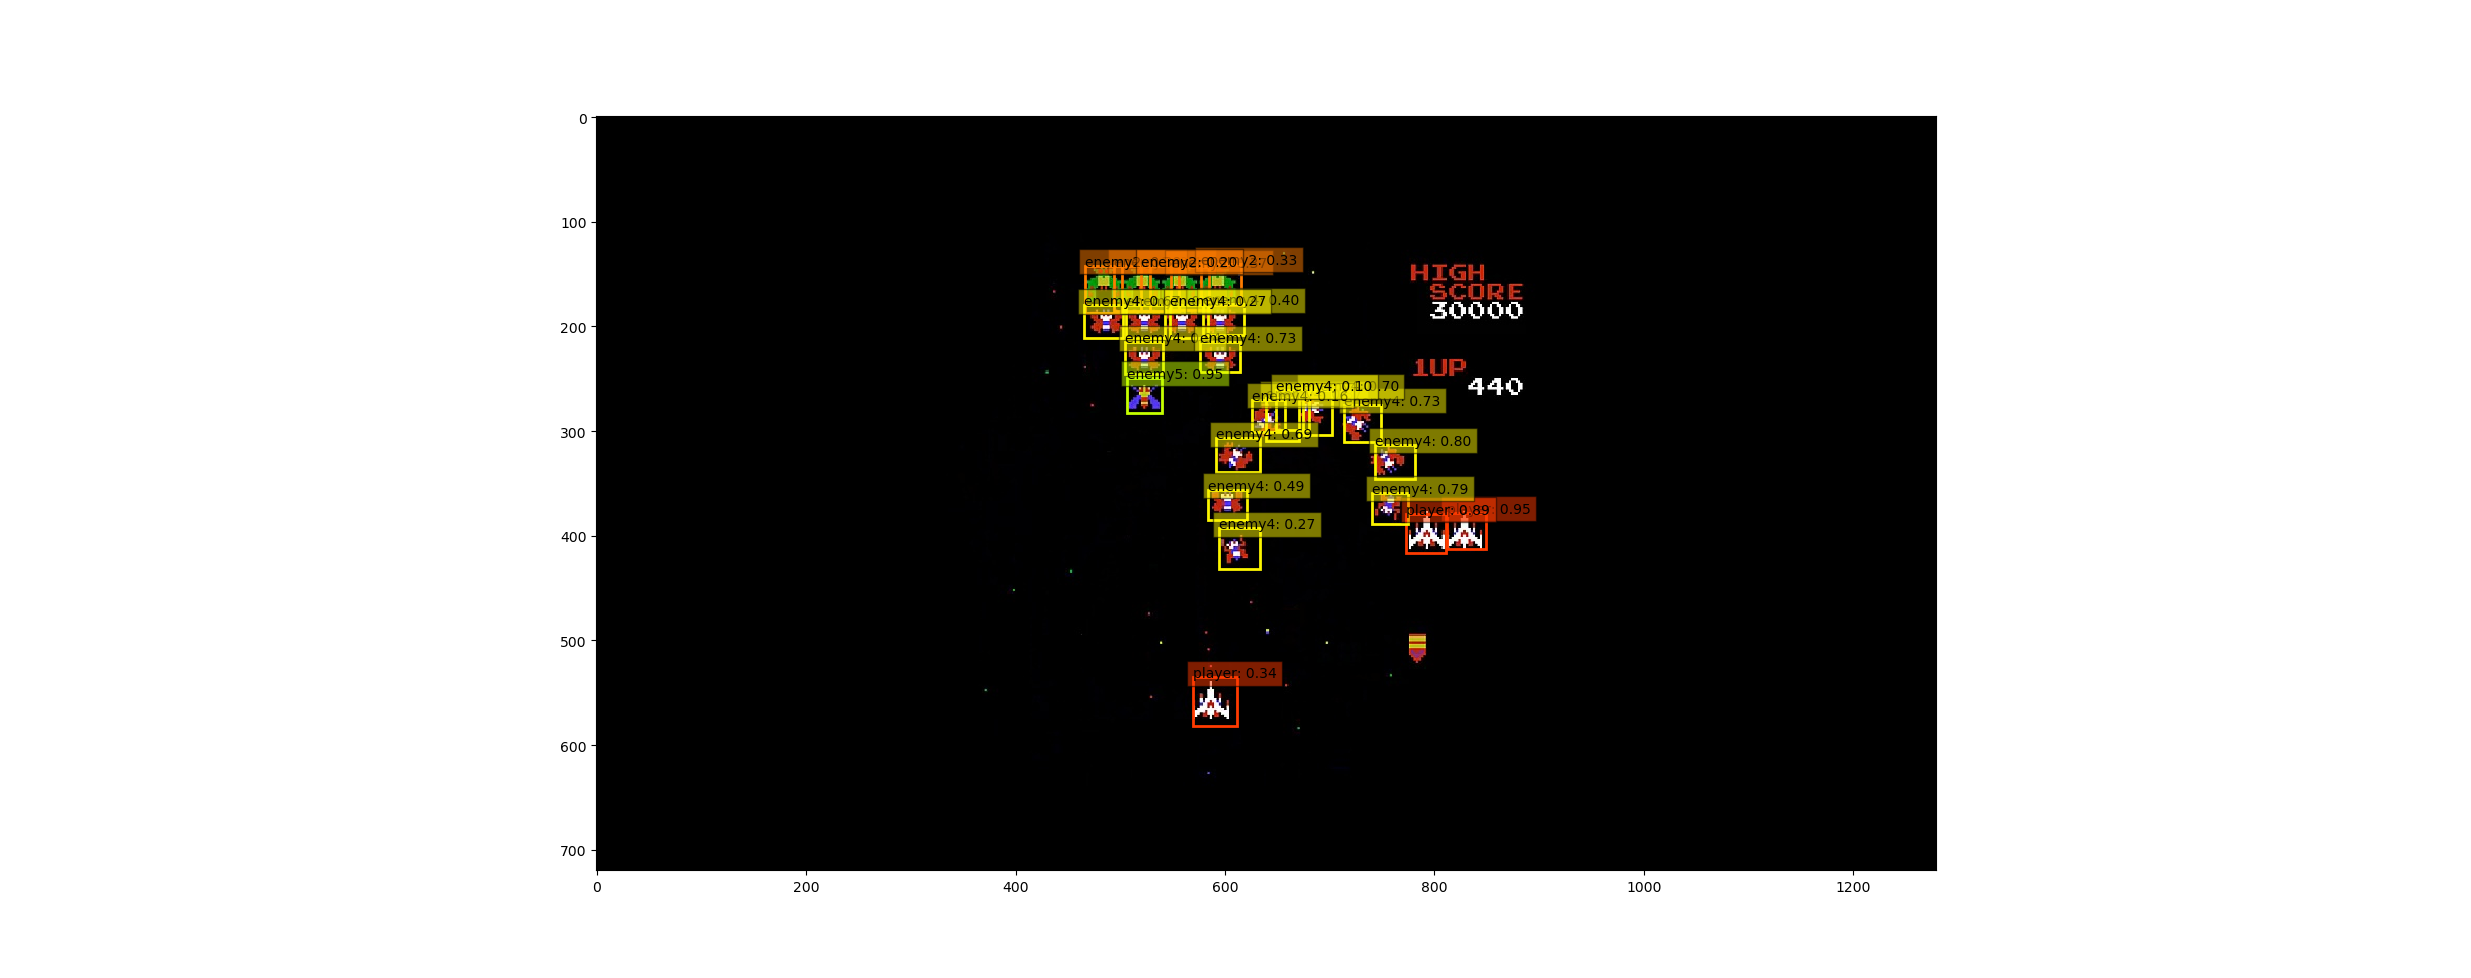
\includegraphics[width=\paperwidth]{d1.eps}}
\end{center}
\subsection{Detection Layer Result Sample 2}
\begin{center}
  \makebox[\textwidth]{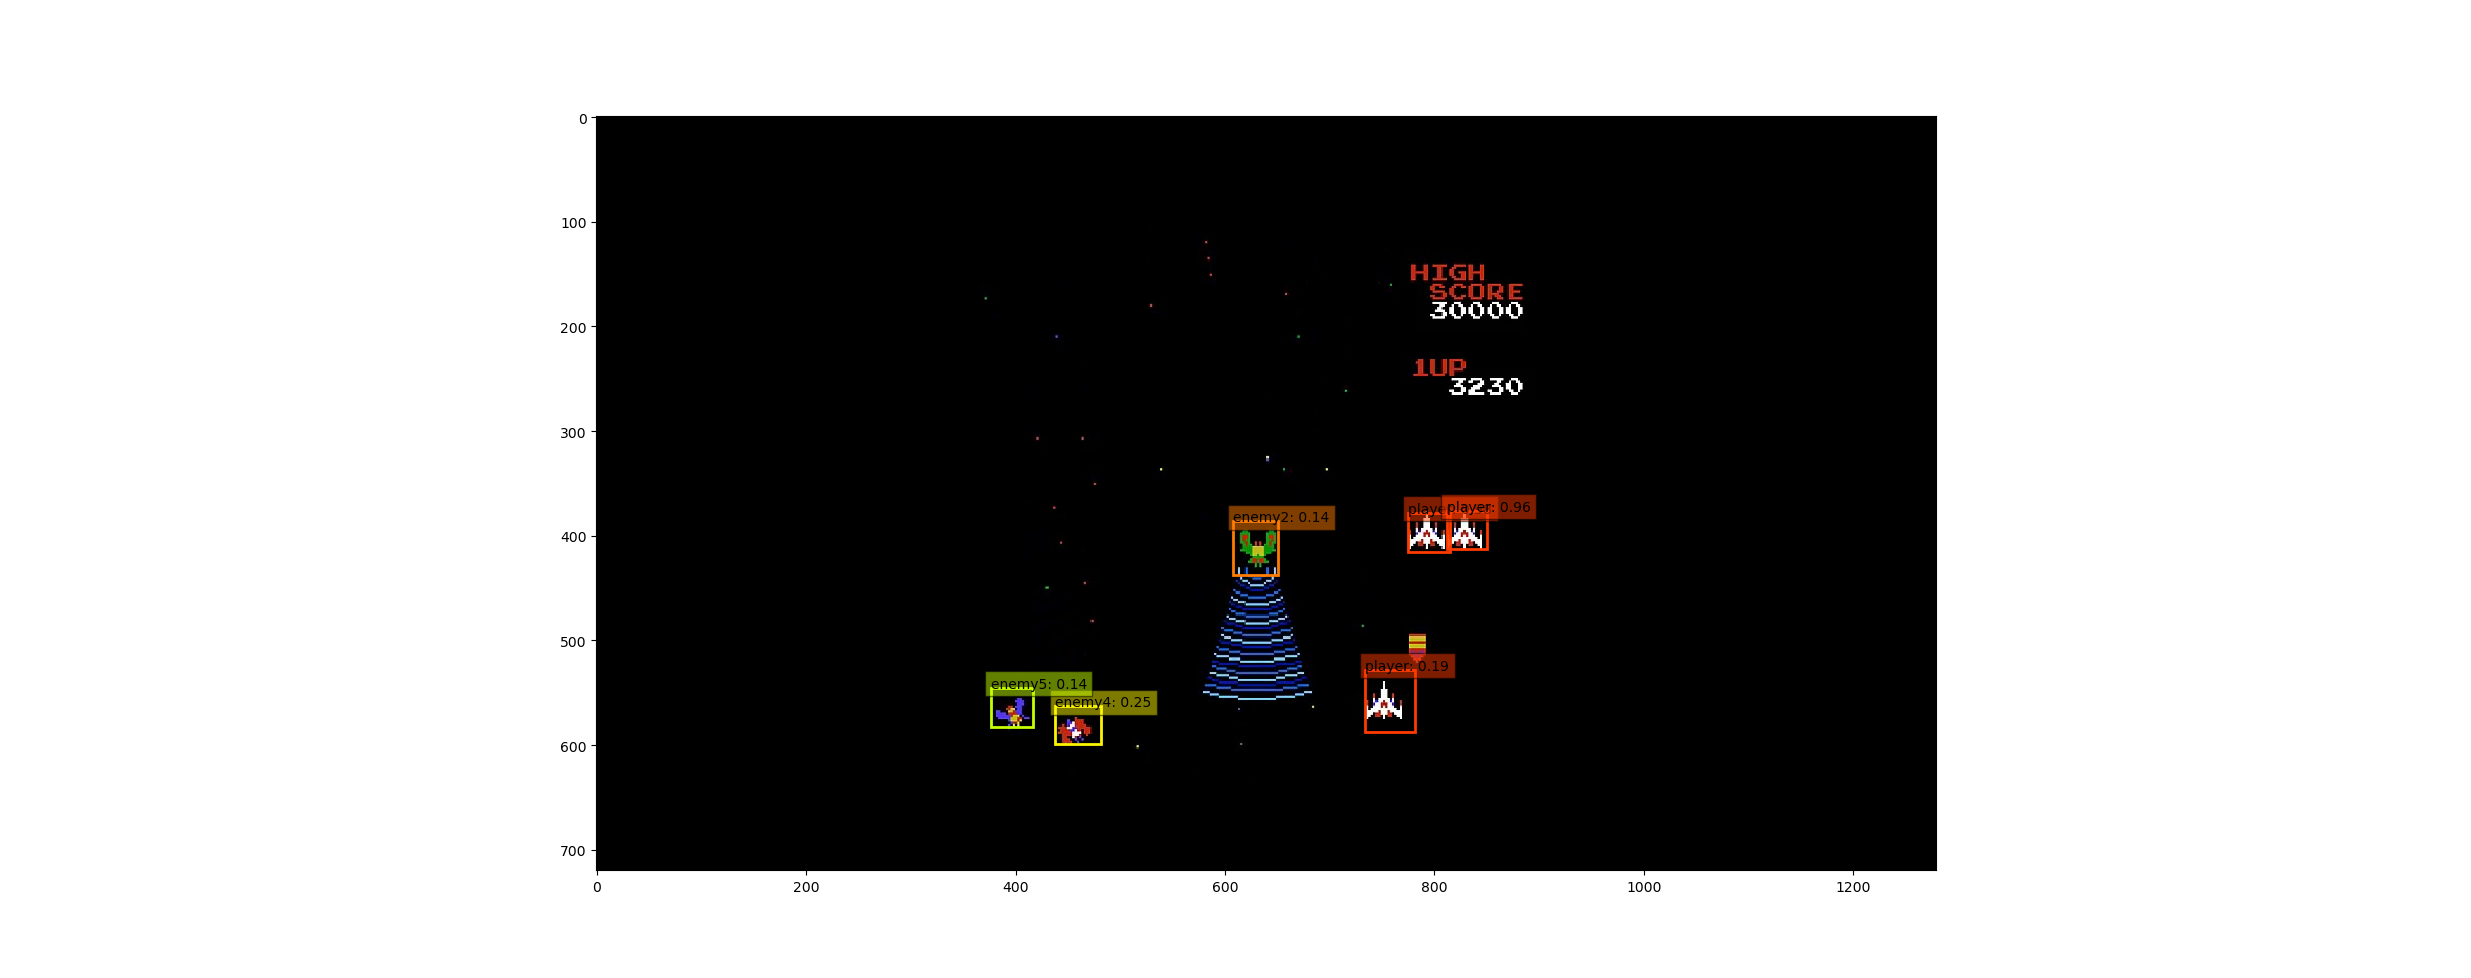
\includegraphics[width=\paperwidth]{d2.eps}}
\end{center}
\subsection{Training plot Loss v.s Accuracy}
\begin{center}
  \makebox[\textwidth]{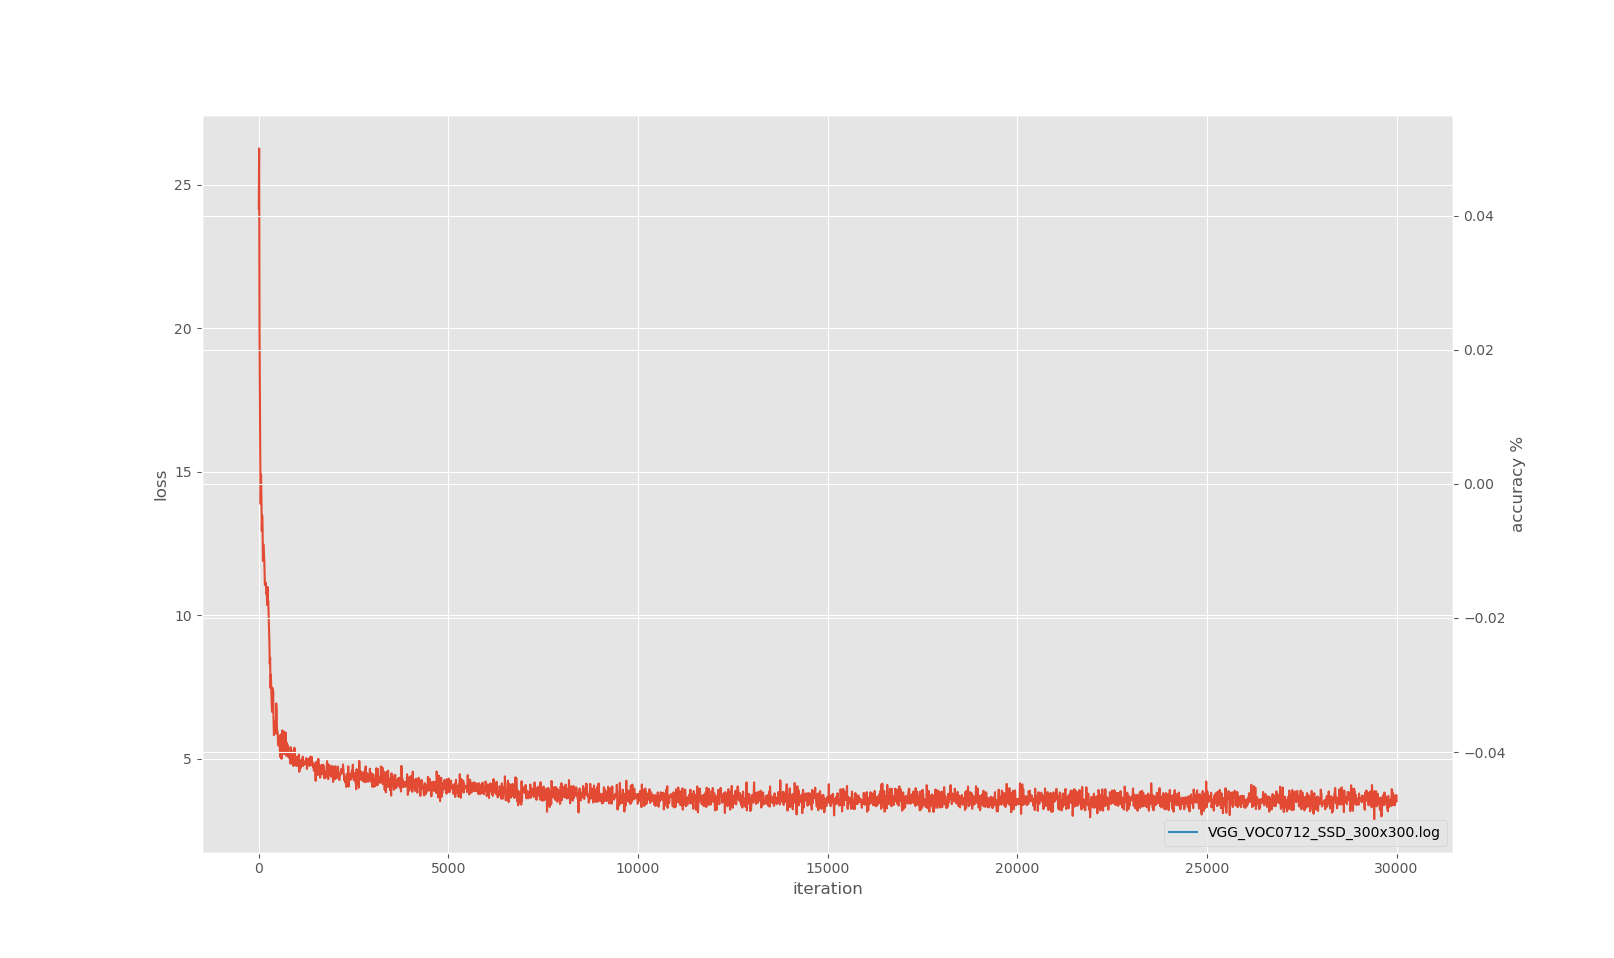
\includegraphics[width=\paperwidth]{plot.eps}}
\end{center}
\subsection{Final Project Setup}
\begin{center}
  \makebox[\textwidth]{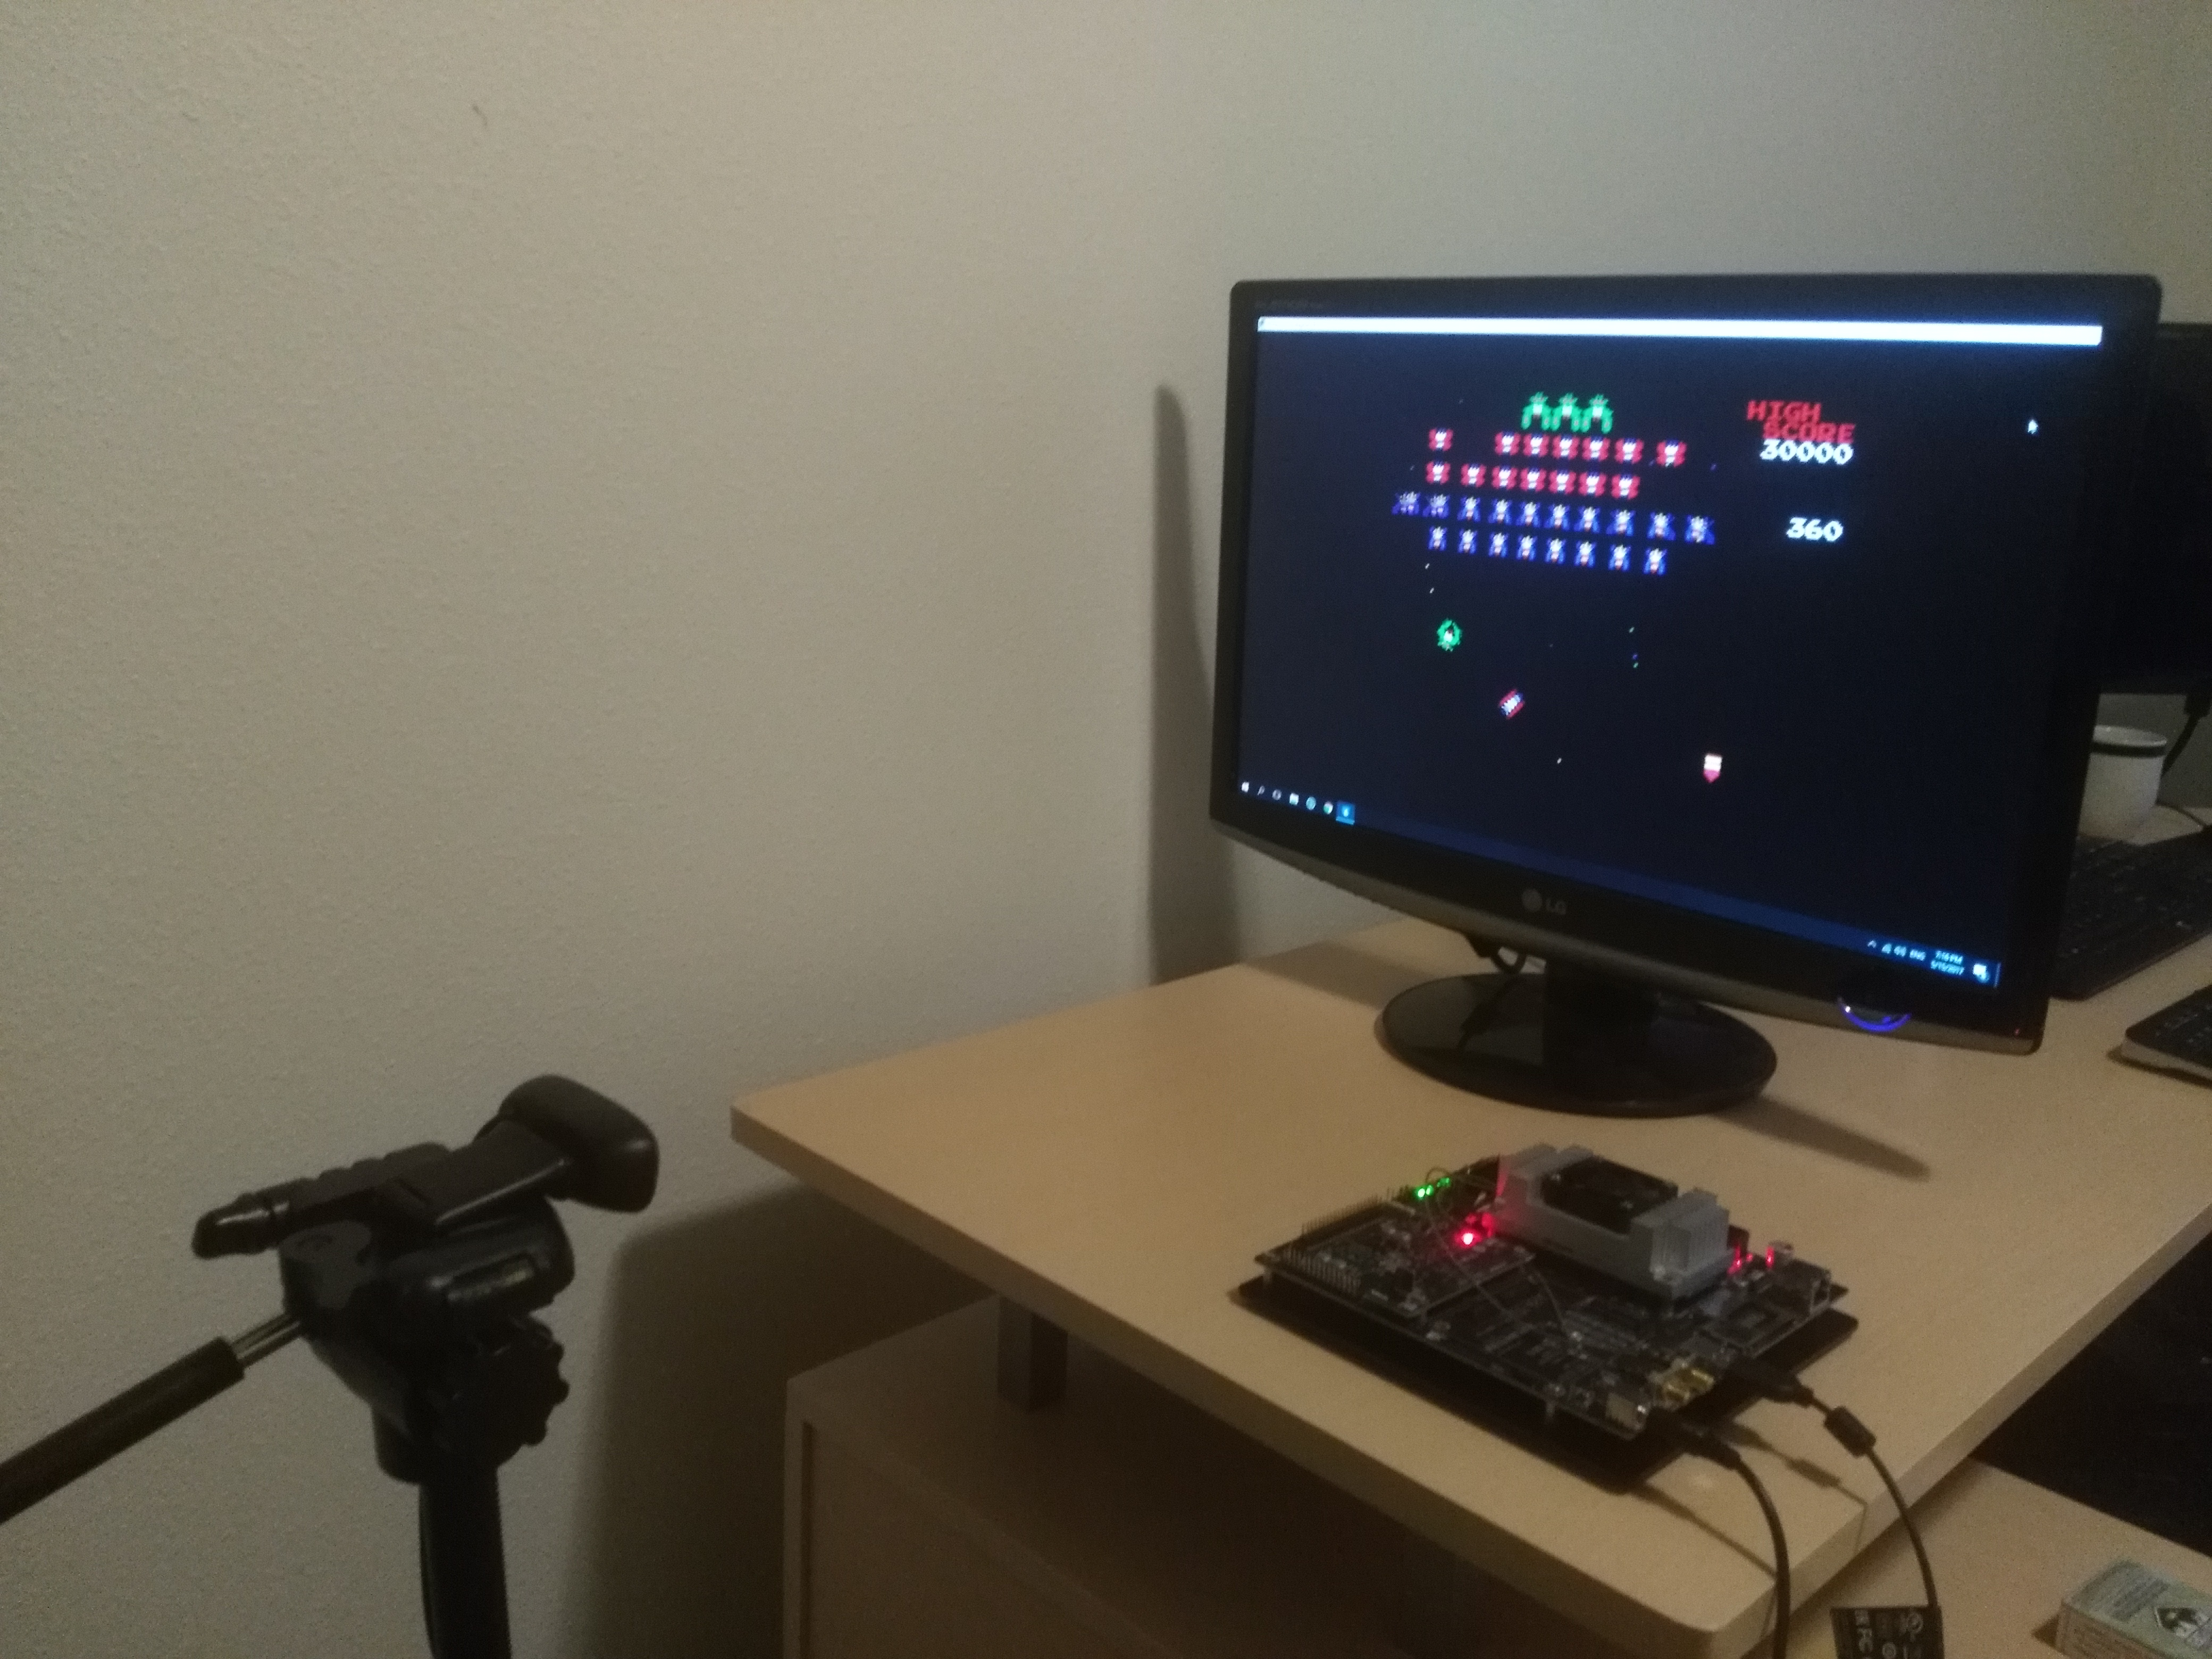
\includegraphics[width=\paperwidth]{setup.eps}}
\end{center}


\end{document}
